\documentclass[a4paper,12pt]{article}
\usepackage[utf8]{inputenc}
\usepackage[brazil]{babel}
\usepackage[top=2.5cm, bottom=2.5cm, left=3cm, right=3cm]{geometry}
\usepackage{setspace}
\usepackage{indentfirst}
\usepackage{multirow}
\usepackage{graphicx}
\usepackage{pgfplots}
\usepackage{amsmath, amsfonts, amssymb, amsthm}
\usepackage{fancyhdr}
\usepackage[scr]{rsfso}
\usepackage{listings}
\usepackage{xcolor}
\usepackage{hyperref}
\hypersetup{
    colorlinks=true,
    linkcolor=black,
    filecolor=magenta,      
    urlcolor=cyan,
    pdftitle={Overleaf Example},
    pdfpagemode=FullScreen,
    }
\urlstyle{same}

\definecolor{codegreen}{rgb}{0,0.6,0}
\definecolor{codegray}{rgb}{0.5,0.5,0.5}
\definecolor{codepurple}{rgb}{0.58,0,0.82}
\definecolor{backcolour}{rgb}{0.95,0.95,0.92}

\lstdefinestyle{mystyle}{
    backgroundcolor=\color{backcolour},   
    commentstyle=\color{codegreen},
    keywordstyle=\color{magenta},
    numberstyle=\tiny\color{codegray},
    stringstyle=\color{codepurple},
    basicstyle=\ttfamily\footnotesize,
    breakatwhitespace=false,         
    breaklines=true,                 
    captionpos=b,                    
    keepspaces=true,                 
    numbers=left,                    
    numbersep=5pt,                  
    showspaces=false,                
    showstringspaces=false,
    showtabs=false,                  
    tabsize=2,
    frame=single,                    % Adiciona uma borda ao redor do código
    framexleftmargin=5mm,            % Margem esquerda da borda
    xleftmargin=5mm,                 % Margem esquerda para quebras de linha
    framesep=2mm,                    % Espaço entre a borda e o código
    columns=fullflexible,            % Melhora o espaçamento entre caracteres
    escapeinside={\%*}{*)},          % Permite inserção de LaTeX dentro do código
}

\lstset{style=mystyle}

\pagestyle{myheadings}
\setlength\parindent{1.25cm}

\begin{document}
%capa
\begin{center}
    \thispagestyle{empty}
    \includegraphics[width=0.9cm]{imgs/ufal-brasão.jpg}\quad
    \includegraphics[width=1.5cm]{imgs/ic- brasão.png}\\
    \large
        \textbf{UNIVERSIDADE FEDERAL DE ALAGOAS}\\
        \textbf{INSTITUTO DE COMPUTAÇÃO}\\
        \textbf{CURSO DE ENGENHARIA DE COMPUTAÇÃO}\\
        \vspace{4cm}
        \textbf{RELATÓRIO DA EXPERIÊNCIA Nº 02}\\
        \textbf{IDENTIFICAÇÃO DE SISTEMAS REPRESENTADOS POR EQUAÇÕES A DIFERENÇAS}\\
        \vspace{4cm}
        \begin{flushright}
            {Tayco Murilo Santos Rodrigues - 17211250}\\
        \end{flushright}
        \vspace{8cm}
        Maceió - AL\\
        2023
\end{center}

%contracapa
\newpage
\begin{center}
    \thispagestyle{empty}
    \large
        Tayco Murilo Santos Rodrigues - 17211250\\
    \vspace{5cm}
    \textbf{IDENTIFICAÇÃO DE SISTEMAS REPRESENTADOS POR EQUAÇÕES A DIFERENÇAS}\\
    \vspace{4cm}
    \begin{flushright}
        \begin{minipage}{ 7.5 cm }
            \normalsize
            Segundo Relatório Parcial apresentado à disciplina de
            Introdução à Identificação de Sistemas, correspondente à
            avaliação do semestre 2023.1 do 10º período do curso de
            Engenharia de Computação da Universidade Federal de
            Alagoas, sob orientação do \textbf{Prof. Ícaro Bezerra Queiroz
            de Araújo.}
        \end{minipage}
    \end{flushright}
    \vspace{8cm}
    Maceió - AL\\
    2023
\end{center}

%resumo
\newpage
\thispagestyle{empty}
\begin{center}
    \large
    \textbf{RESUMO}
\end{center}
Resumo

\vspace{1cm}
\noindent\textbf{Palavras-Chave:}

%lista de símbolos
\newpage
\thispagestyle{empty}
\begin{flushleft}
\Large
\textbf{Lista de Símbolos}
\end{flushleft}



%lista de abreviaturas e siglas
\newpage
\thispagestyle{empty}
\begin{flushleft}
\Large
\textbf{Lista de Abreviaturas e Siglas}
\end{flushleft}

%lista de figuras
\newpage
\onehalfspacing
\thispagestyle{empty}
\listoffigures

\newpage
\onehalfspacing
\thispagestyle{empty}
\lstlistoflistings

%sumário
\newpage
%\onehalfspacing
\thispagestyle{empty}
\tableofcontents

%corpo do texto
\newpage
\onehalfspacing
%Introdução
\section{Introdução}
    \subsection{Contextualização}

    \subsection{Objetivos}
    
    \subsection{Motivação}

    \newpage

%fundamentação teórica
\section{Fundamentação teórica}

%Metodologia
\newpage
\section{Metodologia}

A metodologia do experimento envolve carregar os dados no \texttt{MATLAB}, pré-processamento dos dados se necessário, aplicar algoritmos ou análises específicas e, em seguida, plotar ou apresentar os resultados para interpretação.

\subsection{Sistemas em tempo contínuo (\mathcal{s}) e resposta}\label{3.1}

A resposta ao Degrau unitário de $G_1(s)$ e $G_2(s)$ foi computada, coletada e exibida em um gráfico para melhor visualização. As funções de transferência que definem $G_1(s)$ e $G_2(s)$ são apresentadas abaixo:

\begin{equation*}\label{3.1.1}
G_1(s) = \frac{0.5s^2 + 2s + 2}{s^3 + 3s^2 + 4s + 2} \tag{3.1.1}
\end{equation*}

\begin{equation*}\label{3.1.2}
G_2(s) = \frac{2.5}{s^2 + s + 2.5} \tag{3.1.2}
\end{equation*}
Ambos os sistemas, tiveram sua resposta analisada com relação aos seus polos.

\subsection{Sistemas em tempo discreto (\mathcal{z}) e equações a diferença}\label{3.2}

O próximo passo se deu em discretizar as duas Funções de Transferência usando um período de amostragem de $T_s$ $=$ $0.1s$ e o método de \texttt{Tustin}. O processo foi realizado utilizando a função \texttt{c2d} presente no \texttt{MATLAB}. As Funções de Transferência resultantes são apresentadas abaixo:
\begin{equation*}\label{3.2.1}
G_1(z) = \frac{0.0261z^3 - 0.0166z^2 - 0.0252z + 0.0175}{z^3 - 2.7057z^2 + 2.4484z - 0.7410} \tag{3.2.1}
\end{equation*}

\begin{equation*}\label{3.2.2}
G_2(z) = \frac{0.0059z^2 + 0.0118z + 0.0059}{z^2 - 1.8817z + 0.9053} \tag{3.2.2}
\end{equation*}

Uma vez que temos ambas as funções montadas em \mathcal{z}, podemos explicitar suas equações a diferença. Para $G_1(z)$, temos:
\begin{align}\label{3.2.3}
&0.0261 \cdot u(k-1) - 0.0166 \cdot u(k-2) - 0.0252 \cdot u(k-3) + 0.0175 \cdot u(k-4) = \nonumber \\
&= y(k) - 2.7057 \cdot y(k-1) + 2.4484 \cdot y(k-2) - 0.7410 \cdot y(k-3) \tag{3.2.3}
\end{align}
E para $G_2(z)$:
\begin{align}\label{3.2.4}
& 0.0059 \cdot u(k-1) + 0.0118 \cdot u(k-2) + 0.0059 \cdot u(k-3) = \nonumber \\
& y(k)  - 1.8817 \cdot y(k-1) + 0.9053 \cdot y(k-2) \tag{3.2.4}
\end{align}

A simulação dos sistemas representados nas Funções de Transferência (\ref{3.2.1}) e (\ref{3.2.2}) foi realizada e comparadas com sua resposta contínua. Um degrau unitário foi utilizado como entrada para ambos os sistemas.

\subsection{Gerando uma entrada aleatória}\label{3.3}

Os critérios para gerar a entrada $u(t)$ em questão foram os seguintes:
\begin{itemize}
    \item Distribuição uniforme;
    \item valores no intervalo [ -1,1 ];
    \item Média $0$;
    \item Sem ruído;
    \item Equivalente a $100$ passos de simulação.
\end{itemize}

O código utilizado para gerar a entrada supracitada pode ser visualizado abaixo.

\begin{lstlisting}[language=Matlab, caption=Código responsável por gerar a Entrada aleatória]
% Numero de passos de simulacao
num_steps = 100;

% Gerar valores uniformemente distribuidos no intervalo [0, 1]
u_uniform = rand(1, num_steps);

% Ajustar os valores para o intervalo [-1, 1] com media zero
u_uniform = 2 * u_uniform - 1;

% Plot da entrada uniforme gerada
figure;
stem(u_uniform, 'b', 'LineWidth', 2);
title('Entrada Caracterizada por Distribuicao Uniforme');
xlabel('Tempo (Passo de Simulacao)');
ylabel('Entrada');
grid on;
\end{lstlisting}

O passo seguinte, se deu em gerar valores simulados a partir da Equação a diferença para uma entrada degrau e para a entrada aleatória criada no passo anterior. A entrada aleatória em questão pode ser visualizada de forma gráfica abaixo.

\begin{figure}[h!]\label{fig1}
  \centering
  \includegraphics[width=\textwidth]{imgs/entrada aleatória.png}
  \caption{Exemplo de entrada gerada com o código presente em Listing 1.}
\end{figure}

\subsection{Estimação do Modelo e cálculo do Resíduo}\label{3.4}

Uma vez que podemos gerar uma entrada aleatória como a presente na Figura 1, podemos também, observar e coletar a saída do sistema para esta entrada. Uma vez que a saída em questão foi coletada, podemos fazer uso de métodos de estimação de parâmetros para determinar a função de transferência para este sistema. O método utilizado foi o estimador de mínimos quadrados (\mathcal{EMQ}) e um código exemplo em \texttt{MATLAB} é mostrado abaixo.

\begin{lstlisting}[language=Matlab, caption=Estimador de mínimos quadrados]
for order = 1:max_order
    % Matriz de regressores
    X = zeros(num_data - max_order, order);

    for k = 1:order
        X(:, k) = y_uniform(k:num_data - max_order + k - 1);
    end

    % Dados de saída correspondentes
    y_output = y_uniform(max_order + 1:end);

    % Calcular coeficientes usando EMQ
    theta = X' * X \ X' * y_output;

    % Valores estimados do modelo
    y_estimated = X * theta;
end
\end{lstlisting}

\newpage
O código acima estima parâmetros para um sistema que começa com ordem $1$ e vai até ordem $5$. Com os parâmetros estimados, podemos também calcular o resíduo. De forma que: $\text{Resíduo} = y(k) - y(\hat{k})$. O código responsável por calcular os valores de resíduo e sua média é apresentado abaixo.

\begin{lstlisting}[language=Matlab, caption=Calculo do resíduo e sua média]
for order = 1:max_order
    % Matriz de regressores
    X = zeros(num_data - max_order, order);

    for k = 1:order
        X(:, k) = y_uniform(k:num_data - max_order + k - 1);
    end

    % Dados de saída correspondentes
    y_output = y_uniform(max_order + 1:end);

    % Calcular coeficientes usando EMQ
    theta = X' * X \ X' * y_output;

    % Valores estimados do modelo
    y_estimated = X * theta;

    % Cálculo dos resíduos
    residuals = y_output' - y_estimated;
  
    % Cálculo do valor médio dos resíduos
    mean_residual = mean(residuals);
end
\end{lstlisting}

É fácil ver que o código responsável por calcular o resíduo é o mesmo presente em Listing 2 com o adicional de código presente entre as linhas $18$ e $22$, isso, pois, os passos de execução dos algoritmos são os mesmo até certo ponto. Os resultados obtidos podem ser visualizados no subtópico (\ref{4.4}).

\subsection{Adição de ruído ao Sistema}\label{3.5}

Os critérios para gerar o ruído em questão foram os seguintes:
\begin{itemize}
    \item Gaussiano;
    \item $0.05$ de desvio padrão;
    \item média 0.
\end{itemize}

O ruído em questão é recalculado $100$ vezes, pois o experimento necessita. Para cada ruído calculado os parâmetros do modelo são recalculados, sua média apresentada junto de seu desvio padrão. O código utilizado para realizar esta tarefa com as características supracitadas pode ser visualizado abaixo.

\begin{lstlisting}[language=Matlab, caption=Adição de ruído ao sistema]
for rep = 1:num_repetitions

    %Ruido dinamico
    y_gaussian_dinamic = std_deviation * randn(1, num_data) + mean_value;
    %Ruido estatico
    y_gaussian_static  = std_deviation * randn(1, 1) + mean_value;

    %Adicao de ruido
    noise = . . .;
    out = y + noise;
    
    %Codigo intermediario
    . . .

    % Calculo da media
    m_value = mean(theta);

    % Calculo do desvio padrao
    s_deviation = std(theta);

    % Display coefficients and difference equation
    . . .
end
\end{lstlisting}

O código acima apresenta duas formas de se adicionar ruído ao Sistema. O ruído estático(Adicionado de uma vez ao sistema):
\begin{equation*}
    Y(k) = Y(k) + E(k) \tag{3.5.1}
\end{equation*}
E o ruído dinâmico(Adicionado a cada amostragem):
\begin{equation*}
    y(k) = y(k) + e(k) \tag{3.5.2}
\end{equation*}
Ambos são apresentados respectivamente nas linhas $4$ e $6$ do código presente em Listing 4.

\subsection{Validação dos Modelos}\label{3.6}

Neste experimento, foi realizada a validação dos modelos obtidos anteriormente a partir de uma entrada em forma de senoide, por meio de três métodos estatísticos: simulação com um conjunto diferente de dados de entrada e o cálculo do erro quadrático, coeficiente de correlação múltipla e a razão sinal-ruído (S/R). O objetivo é avaliar a capacidade de cada modelo em se ajustar aos dados reais e determinar quão bem eles representam o comportamento do sistema. O código utilizado para gerar ($u(t)$) e o sinal em questão podem ser visualizados abaixo.

\begin{figure}[h!]\label{validacao-sinal}
  \centering
  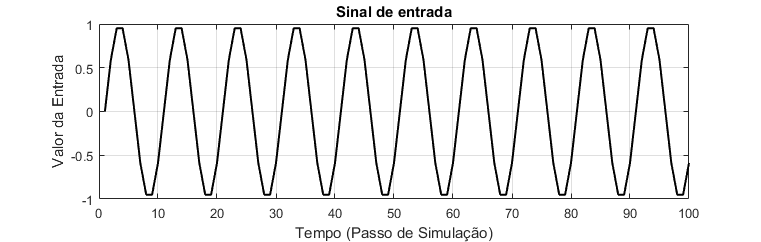
\includegraphics[width=\textwidth]{imgs/val-sinal-entrada.png}
  \caption{Sinal de entrada Utilizado para validação.}
\end{figure}

\begin{lstlisting}[language=Matlab, caption=$u(t)$ para validação]
% Tempo de amostragem
T = 0.1;

% Número de passos de simulação
num_steps = 100;

t = 0:T:(num_steps-1)*T;  % Vetor de tempos
u = sin(2 * pi * t); % Sinal de entrada(senoide)
\end{lstlisting}

Os modelos de primeira até quinta ordem estimados foram submetidos à entrada em questão, e suas saídas foram submetidas ao ruído gaussiano \textbf{dinâmico}, criado no subtópico \ref{3.5}. A escolha da aplicação do ruído dinâmico se deu com base nos resultados preliminares obtidos antes da adição do mesmo, uma vez que o sinal de saída submetido ao ruído \textbf{estático} sofreu \textbf{poucas alterações}. 

Aplicamos cada um dos modelos obtidos anteriormente a esses novos dados de entrada e calculamos o erro quadrático entre as saídas estimadas e as saídas reais do sistema. O código responsável por calcular a soma dos erros ao quadrado é mostrado abaixo.
\begin{lstlisting}[language=Matlab, caption=Calculo do somatório dos erros ao quadrado.]
% Cálculo do somatório do erro quadrático
se = sum((y_output' - y_estimated).^2);
disp(['Somatório do Erro Quadrático: ' num2str(se)]);
\end{lstlisting}

Em seguida, Calculamos o coeficiente de correlação múltipla para cada modelo, comparando as saídas estimadas com as saídas reais do sistema. O código responsável por calcular o coeficiente de correlação múltipla é mostrado abaixo.
\begin{lstlisting}[language=Matlab, caption=Calculo do coeficiente de correlação multipla.]
% Cálculo do coeficiente de correlação múltipla
y_mean = mean(y_output);
ss_total = sum((y_output' - y_mean).^2);
ss_residual = sum((y_output' - y_estimated).^2);
r_squared = 1 - ss_residual / ss_total;
disp(['Coeficiente de Correlação Múltipla: ' num2str(r_squared)]);
\end{lstlisting}

Por fim, a razão sinal-ruído foi obtida, a mesma é uma métrica que avalia a proporção do sinal (informação útil) em relação ao ruído (variabilidade não explicada) nos dados. Calculamos a S/R para as saídas estimadas e reais de cada modelo. Quanto maior a S/R, mais informações relevantes o modelo está capturando e menos influência o ruído exerce. O código responsável por calcular a relação sinal-ruido é mostrado abaixo.
\begin{lstlisting}[language=Matlab, caption=Calculo da relação sinal-ruido.]
% Cálculo razão sinal-ruido
signal_power = sum(y_estimated.^2);
noise_power  = sum(noise.^2);
snr_value = signal_power / noise_power;
snr_value = 10 * log10(snr_value);
disp(['Razão Sinal-Ruído (SNR): ' num2str(snr_value)]);
\end{lstlisting}

Após a aplicação dos modelos aos novos dados de entrada e o cálculo das métricas, foram gerados gráficos que comparam as saídas reais do sistema com as saídas estimadas por cada modelo. Observamos a sobreposição das curvas para avaliar visualmente o ajuste. Os resultados desses métodos de validação nos permitirão avaliar a qualidade de ajuste de cada modelo aos dados reais. Modelos que apresentam baixo erro quadrático, alto coeficiente de correlação múltipla e alta razão S/R são considerados mais adequados para representar o comportamento do sistema.

\subsection{Identificação de Modelos ARX e ARMAX}\label{3.7}

A metodologia adotada consiste em identificar modelos matemáticos para os Conjuntos de Dados 1, 2, 3 e 4 por meio dos modelos ARX e ARMAX. As ordens dos modelos variam de 1 a 5. O processo de identificação ocorre em duas fases: estimação e validação.

Na fase de estimação, os modelos ARX e ARMAX são ajustados aos dados. O modelo ARX é definido pela equação:

\begin{equation*}\label{3.7.1}
    y(t) = \sum_{i=1}^{p} a_i y(t-i) + \sum_{j=1}^{q} b_j u(t-j) + e(t) \tag{3.7.1}
\end{equation*}

Enquanto o modelo ARMAX incorpora termos de médias móveis:

\begin{equation*}\label{3.7.2}
    y(t) = \sum_{i=1}^{p} a_i y(t-i) + \sum_{j=1}^{q} b_j u(t-j) + \sum_{k=1}^{r} c_k e(t-k) \tag{3.7.2}
\end{equation*}

Na fase de validação, os modelos ajustados são testados. O desempenho de cada modelo é avaliado calculando o erro médio quadrático (EMQ), dado por:

\begin{equation}
    EMQ = \frac{1}{N} \sum_{t=1}^{N} (y_{\text{real}}(t) - y_{\text{previsto}}(t))^2 \tag{3.7.3}
\end{equation}

O modelo que apresentar o menor EMQ pode ser considerado aquele com melhor ajuste aos dados. Já para os conjuntos 3 e 4 foi adicionada mais uma etapa de validação para fins de verificar se os modelos variam com o tempo, isso pode ser feito plotando o comportamento dos regressores (coeficientes dos termos autorregressivos e exógenos) ao longo do tempo. Isso ajuda a entender a evolução das influências das variáveis no processo.

%Resultado
\newpage
\section{Resultados}

\subsection{Resposta dos Sistemas em Malha Aberta}\label{4.1}

Como descrito no subtópico (\ref{3.1}), os Sistemas em malha aberta representados pelas funções de transferência (\ref{3.1.1}) e (\ref{3.1.2}) foram submetidos à entra degrau e o resultado é apresentado abaixo:

\begin{figure}[h!]\label{fig2}
  \centering
  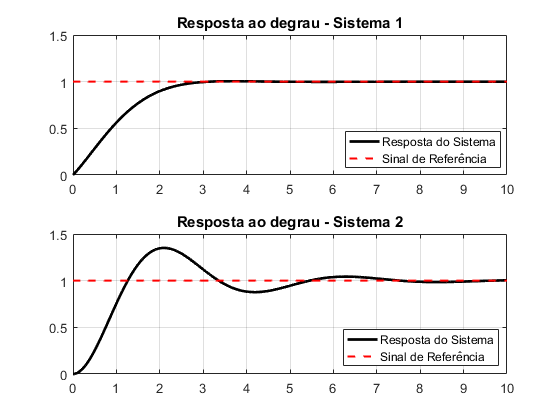
\includegraphics[width=\textwidth]{imgs/comparativo-1.png}
  \caption{Resposta dos Sistemas (\ref{3.1.1}) e (\ref{3.1.2}) ao Degrau unitário.}
\end{figure}

Podemos notar que o Sistema $G_1(s)$ apresenta uma resposta próxima a um sistema de \textbf{primeira ordem}, enquanto o Sistema $G_2(s)$ apresenta uma resposta próxima a um sistema de \textbf{segunda ordem subamortecido}. Os polos de ambos são apresentados abaixo:

\begin{equation*}
\text{Polos do Sistema 1:} \quad -1.0 + 1.0i, \quad -1.0 - 1.0i, \quad -1.0
\end{equation*}
\begin{equation*}
\text{Polos do Sistema 2:} \quad -0.5 + 1.5i, \quad -0.5 - 1.5i
\end{equation*}

Os polos de um sistema de controle têm um impacto direto no desempenho do sistema. Nos próximos subtópicos são apresentados uma caracterização dos sistemas \ref{3.1.1} e \ref{3.1.2} com base nos critérios de desempenho observados em seus polos.

\subsubsection{Sistema \ref{3.1.1}}\label{4.4.1.1}

\textbf{Tempo de Resposta:} Os polos reais ($-1$) indicam que o sistema terá uma resposta relativamente rápida, com um tempo de subida menor. A parte imaginária pequena dos polos indica que as oscilações serão amortecidas.

\textbf{Estabilidade:} Todos os polos estão localizados no semiplano esquerdo do plano complexo, o que indica que o sistema é estável, pois todos os polos têm partes reais negativas.

\textbf{Amortecimento:} Os polos complexos conjugados ($-1 + 1i$, $-1 - 1i$) sugerem um amortecimento moderado das oscilações, resultando em uma resposta suave.

\textbf{Oscilações:} Os polos complexos conjugados também indicam oscilações na resposta, mas o fato de terem uma parte imaginária relativamente pequena sugere que as oscilações serão controladas.

\subsubsection{Sistema \ref{3.1.2}}\label{4.4.1.2}

\textbf{Tempo de Resposta:} Os polos complexos conjugados com uma parte real negativa indicam um tempo de resposta mais rápido em comparação com um sistema puramente real.

\textbf{Estabilidade:} Assim como o Sistema 1, todos os polos estão no semiplano esquerdo, garantindo estabilidade.

\textbf{Amortecimento:} A parte imaginária dos polos complexos sugere oscilações, mas o fato de ter uma parte real negativa indica um amortecimento razoável.

\textbf{Oscilações:} A parte imaginária dos polos indica a presença de oscilações na resposta, mas a combinação com a parte real negativa implica que essas oscilações são controladas.\\

\noindent Em resumo, ambos os sistemas parecem ter respostas controladas e estáveis, com oscilações moderadas. O Sistema 1 parece ter um amortecimento um pouco mais forte devido aos polos reais próximos, enquanto o Sistema 2 tem polos complexos conjugados que resultam em uma resposta mais rápida.

\subsection{Resposta dos Sistemas Discretizados}\label{4.2}

As simulações apresentadas abaixo foram realizadas utilizando as funções de transferência em $z$, para os sistemas $G_1$ e $G_2$, respectivamente apresentados em (\ref{3.2.1}) e (\ref{3.2.2}). O métodos de discretização utilizado junto da entrada $u(t)$ para ambos os sistemas podem ser visualizadas revisitando o tópico \ref{3.2}.

\begin{figure}[h!]\label{fig3}
  \centering
  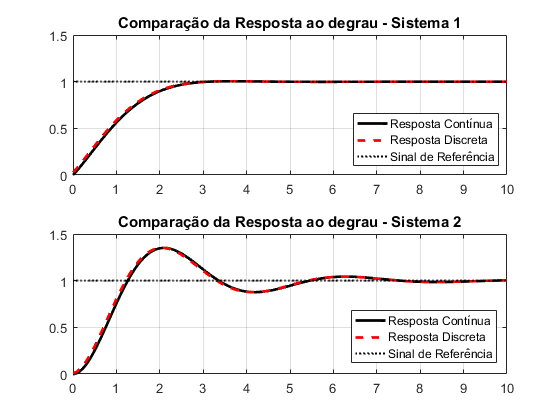
\includegraphics[width=\textwidth]{imgs/comparativo-2.png}
  \caption{Comparativo entre $G(s)$ e $G(z)$ para ambos os sistemas.}
\end{figure}

A comparação entre um sistema discretizado usando o método de \texttt{Tustin} com um período de amostragem de $0.1s$ e o mesmo sistema contínuo, quando suas saídas não diferem significativamente, ressalta a eficácia da discretização em preservar o comportamento dinâmico e a resposta em frequência do sistema contínuo. Esse resultado sugere que o método de \texttt{Tustin}, ao escolher um período de amostragem apropriado, consegue capturar fielmente a natureza do sistema contínuo, sendo uma abordagem valiosa para análise e controle.

\subsection{Resposta à entrada aleatória}\label{4.3}

Utilizando a entrada gerada no passo apresentado no tópico (\ref{3.3}) em conjunto de uma entrada degrau podemos observar e interpretar a saída do sistema. As saídas em questão podem ser observadas abaixo. 

\begin{figure}[h!]\label{fig4}
  \centering
  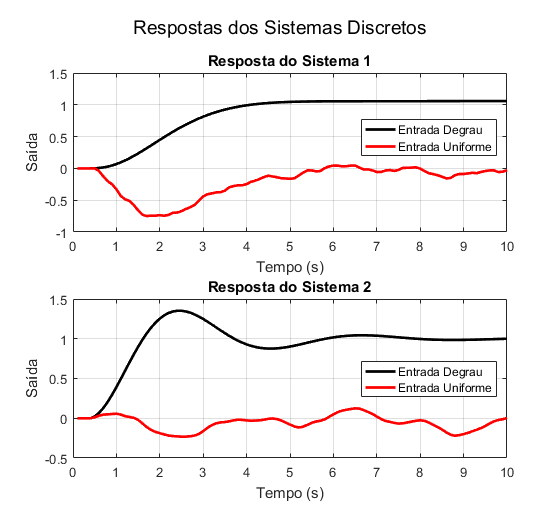
\includegraphics[width=\textwidth]{imgs/comparativo-3.png}
  \caption{Comparativo para as diferentes entradas para $G(z)$.}
\end{figure}

A resposta do \textbf{Sistema 1 discreto} para a entrada uniforme mostra que, inicialmente, a saída segue a entrada, mas com o tempo, a resposta começa a oscilar e se estabiliza em um valor próximo a zero. Isso acontece porque os polos complexos conjugados do Sistema 1 têm uma parte real negativa, o que resulta em oscilações amortecidas. A resposta suave indica que as oscilações são controladas e a saída eventualmente converge para um valor próximo a zero, que é a média da entrada uniforme.

A resposta do \textbf{Sistema 2 discreto} para a entrada uniforme também mostra um comportamento oscilatório, mas em uma escala menor em comparação com o Sistema 1. Isso ocorre porque o Sistema 2 possui apenas um polo complexo com parte real negativa. Essa parte real negativa faz com que a resposta se mova em direção a zero ao longo do tempo. As oscilações na resposta são causadas pelo polo complexo. Assim como no Sistema 1, essas oscilações estão amortecidas e a saída converge para um valor próximo a zero. Agora, para os sistemas contínuos, temos as seguintes saídas.

\begin{figure}[h!]\label{fig5}
  \centering
  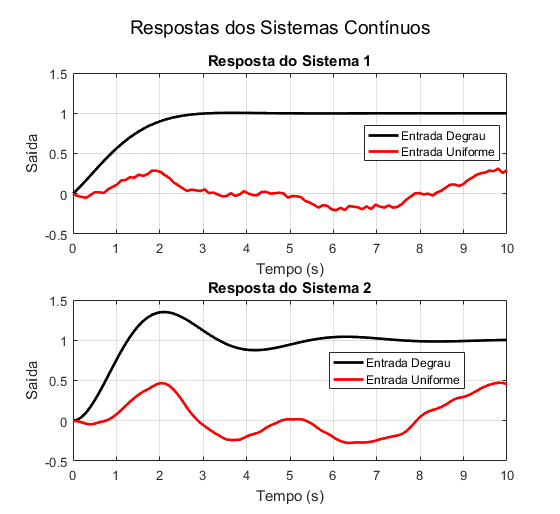
\includegraphics[width=\textwidth]{imgs/comparativo-4.png}
  \caption{Comparativo para as diferentes entradas para $G(s)$.}
\end{figure}

A resposta do \textbf{Sistema 1 contínuo} para a entrada uniforme exibe uma resposta transitória inicial à entrada e, eventualmente, converge para um valor próximo a zero. Isso ocorre porque os polos do Sistema 1 têm partes reais negativas, o que indica uma resposta estável e a tendência da saída em retornar ao equilíbrio (zero). A resposta transitória inicial é uma característica comum de sistemas de primeira e segunda ordem. A convergência para zero ocorre devido à natureza estável dos polos.

A resposta do \textbf{Sistema 2 contínuo} para a entrada uniforme também mostra uma resposta transitória inicial, seguida por uma convergência para zero. A presença de um único polo com parte real negativa no Sistema 2 faz com que a saída retorne ao equilíbrio de maneira suave e estável. A resposta transitória inicial é uma consequência natural da mudança da entrada e é observada em sistemas de primeira ordem.

\subsection{Parâmetros encontrados utilizando EMQ}\label{4.4}

\subsubsection{Sistema \ref{3.2.1}}
As seguintes equações a diferença foram encontradas utilizando o método EMQ apresentado em (\ref{3.4}).\\

\noindent \textbf{Modelo de Ordem 1:}
\begin{equation*}
    y(k) = 0.92 \cdot u(k-1)\tag{4.4.1.1}
\end{equation*}
Nesse modelo de primeira ordem, os resíduos são principalmente pequenos, o que sugere que o modelo está bem calibrado para os dados. Mas devido ao baixo número de parâmetros, acaba sofrendo uma defasagem quando comparado ao modelo original.

\begin{figure}[h!]
\begin{center}
	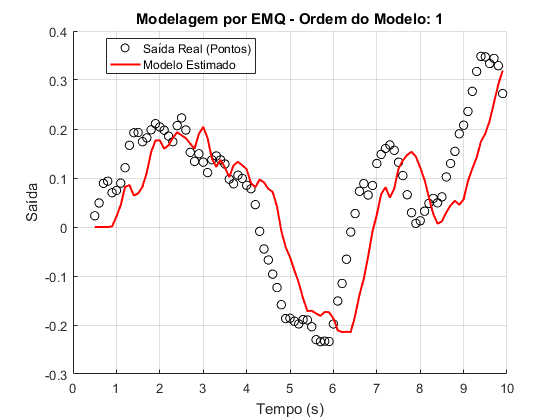
\includegraphics[height=5.4cm]{imgs/emq-1.png} \quad
	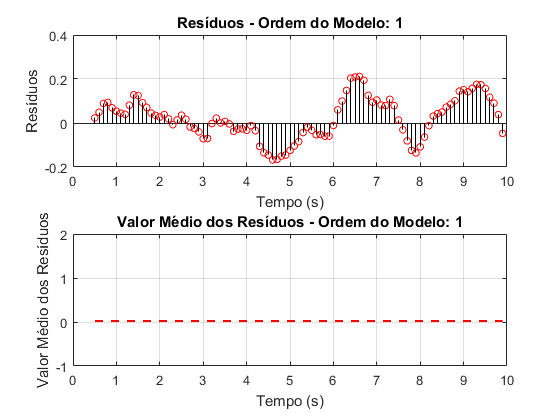
\includegraphics[height=5.4cm]{imgs/residuo-1.png}
\caption{Resultados para $G_1(z)$ de ordem $1$} \label{fig6}
\end{center}
\end{figure}

\noindent \textbf{Modelo de Ordem 2:}
\begin{equation*}
    y(k) = -1.82 \cdot u(k-1) + 2.70 \cdot u(k-2)\tag{4.4.1.2}
\end{equation*}
Nesse modelo de segunda ordem, os resíduos têm algumas flutuações, mas o valor médio dos resíduos é relativamente baixo ($0.0143$), indicando que o modelo ainda está se ajustando bem aos dados.

\begin{figure}[h!]
\begin{center}
	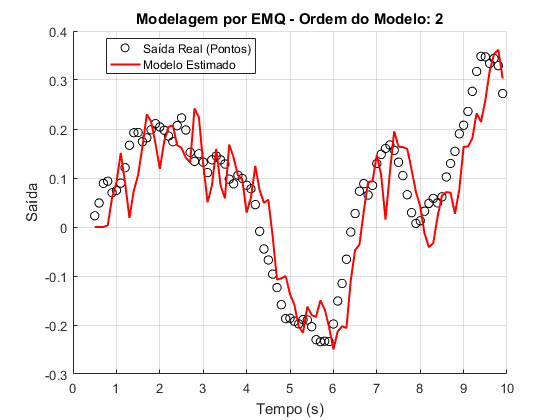
\includegraphics[height=5.4cm]{imgs/emq-2.png} \quad
	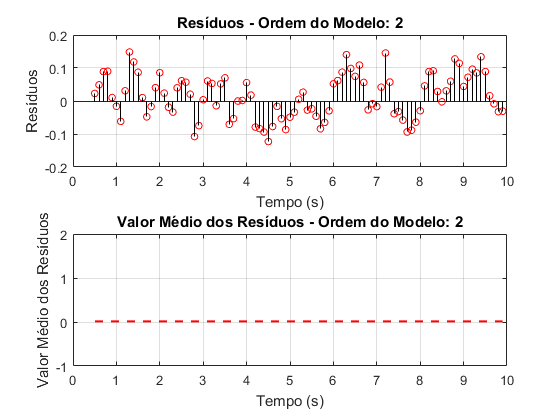
\includegraphics[height=5.4cm]{imgs/residuo-2.png}
\caption{Resultados para $G_1(z)$ de ordem $2$} \label{fig7}
\end{center}
\end{figure}

\newpage
\noindent \textbf{Modelo de Ordem 3:}
\begin{equation*}
y(k) = -0.13 \cdot u(k-1) - 1.30 \cdot u(k-2) + 2.34 \cdot u(k-3)\tag{4.4.1.3}
\end{equation*}
Nesse modelo, os resíduos são pequenos e variam ao longo do tempo. O valor médio dos resíduos é ainda menor ($0.0097$), indicando um ajuste razoável aos dados.

\begin{figure}[h!]
\begin{center}
	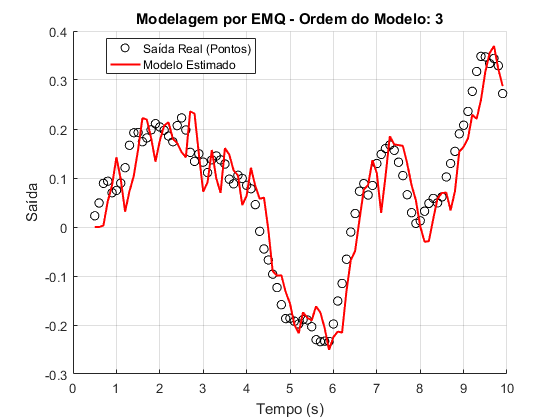
\includegraphics[height=5.4cm]{imgs/emq-3.png} \quad
	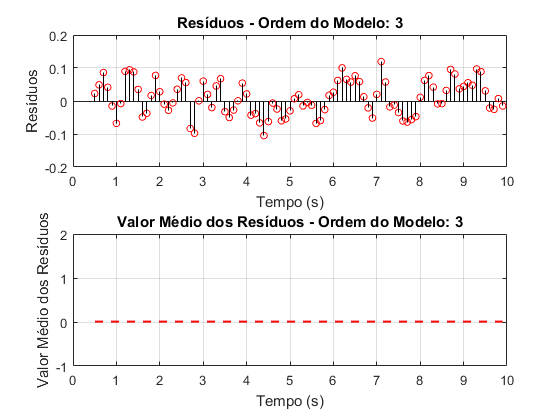
\includegraphics[height=5.4cm]{imgs/residuo-3.png}
\caption{Resultados para $G_1(z)$ de ordem $3$} \label{fig8}
\end{center}
\end{figure}

\noindent \textbf{Modelo de Ordem 4:}
\begin{equation*}
   y(k) = -0.56 \cdot u(k-1) + 0.93 \cdot u(k-2) - 1.57 \cdot u(k-3) + 2.13 \cdot u(k-4)\tag{4.4.1.4}
\end{equation*}
Nesse modelo de quarta ordem, os resíduos variam consideravelmente e parecem ter mais flutuações do que os modelos anteriores. O valor médio dos resíduos ainda é relativamente baixo ($0.0057$), sugerindo um ajuste razoável aos dados.

\begin{figure}[h!]
\begin{center}
	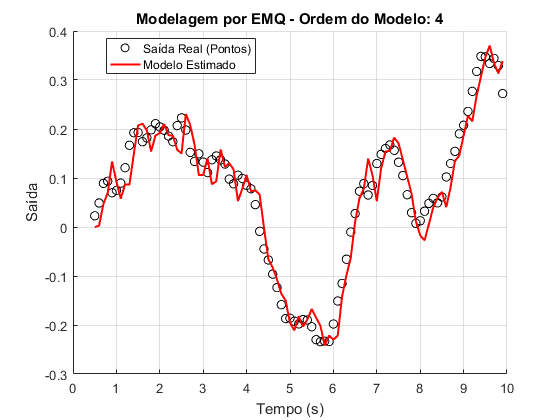
\includegraphics[height=5.4cm]{imgs/emq-4.png} \quad
	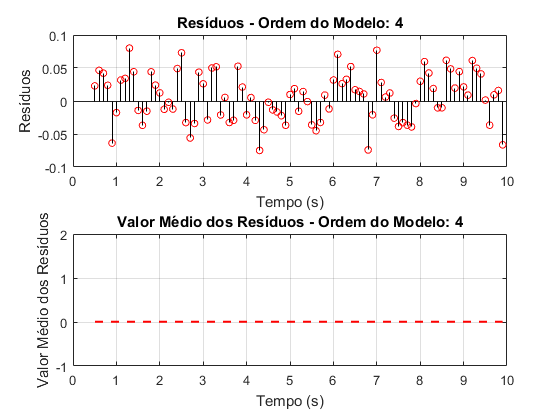
\includegraphics[height=5.4cm]{imgs/residuo-4.png}
\caption{Resultados para $G_1(z)$ de ordem $4$} \label{fig9}
\end{center}
\end{figure}

\newpage
\noindent \textbf{Modelo de Ordem 5:}
\begin{equation*}
    y(k) = 0.17 \cdot u(k-1) - 0.71 \cdot u(k-2) + 1.13 \cdot u(k-3) - 1.57 \cdot u(k-4) + 1.96 \cdot u(k-5)\tag{4.4.1.5}
\end{equation*}
Nesse modelo de quinta ordem, os resíduos têm menos flutuações em comparação com o modelo de quarta ordem. O valor médio dos resíduos é muito baixo ($0.0018$), sugerindo um bom ajuste aos dados.

\begin{figure}[h!]
\begin{center}
	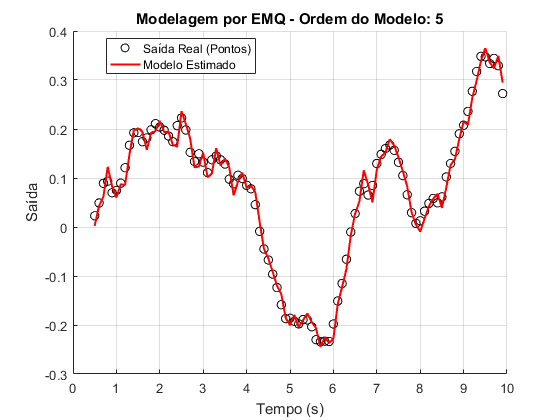
\includegraphics[height=5.4cm]{imgs/emq-5.png} \quad
	\includegraphics[height=5.4cm]{imgs/resíduo-5.png}
\caption{Resultados para $G_1(z)$ de ordem $5$} \label{fig10}
\end{center}
\end{figure}

No geral, os modelos parecem estar se ajustando razoavelmente bem aos dados simulados. Modelos de ordem mais baixa tendem a ter resíduos um pouco mais variáveis, enquanto modelos de ordem mais alta têm resíduos mais suaves. O valor médio dos resíduos em todos os casos é relativamente baixo, indicando um ajuste satisfatório.

\subsubsection{Sistema \ref{3.2.2}}

As seguintes equações a diferença foram encontradas utilizando o método EMQ apresentado em (\ref{3.4}).\\

\noindent \textbf{Modelo de Ordem 1:}
\begin{equation*}
   y(k) = 0.78 \cdot u(k-1)\tag{4.4.2.1}
\end{equation*}
Os resíduos mostram uma tendência geral de estar próximos de zero, o que sugere que o modelo de ordem 1 ajustou razoavelmente bem os dados.

\begin{figure}[h!]
\begin{center}
	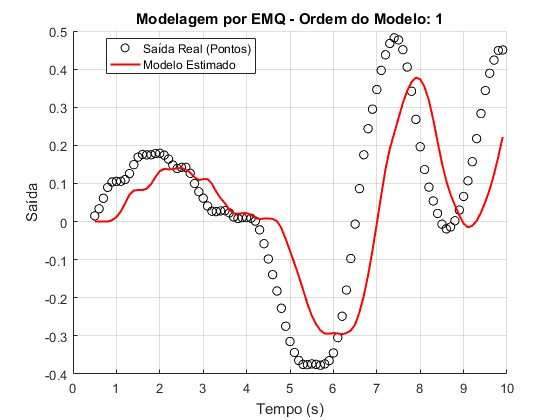
\includegraphics[height=5.4cm]{imgs/emq2-1.png} \quad
	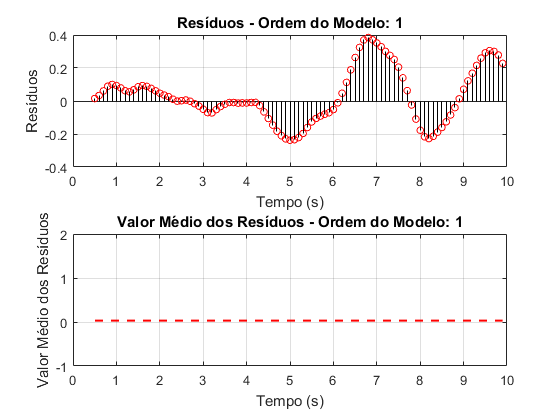
\includegraphics[height=5.4cm]{imgs/residuo2-1.png}
\caption{Resultados para $G_2(z)$ de ordem $1$} \label{fig11}
\end{center}
\end{figure}
\newpage
\noindent \textbf{Modelo de Ordem 2:}
\begin{equation*}
    y(k) = -3.46 \cdot u(k-1) + 4.24 \cdot u(k-2)\tag{4.4.2.2}
\end{equation*}
Os resíduos parecem variar mais do que no modelo de ordem 1, o que pode indicar que o modelo de ordem 2 está ajustando os dados com mais detalhes.

\begin{figure}[h!]
\begin{center}
	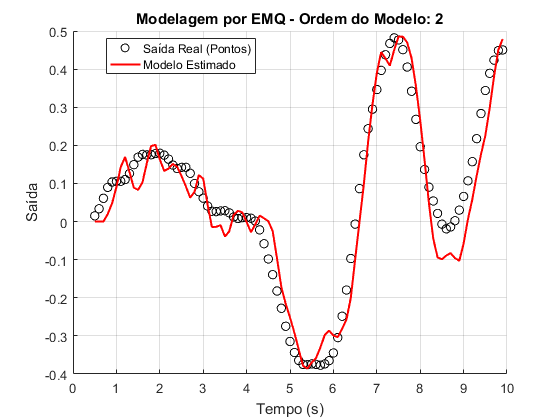
\includegraphics[height=5.4cm]{imgs/emq2-2.png} \quad
	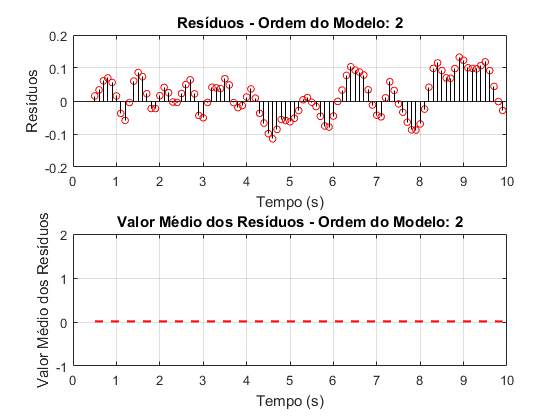
\includegraphics[height=5.4cm]{imgs/residuo2-2.png}
\caption{Resultados para $G_2(z)$ de ordem $2$} \label{fig12}
\end{center}
\end{figure}

\noindent \textbf{Modelo de Ordem 3:}
\begin{equation*}
   y(k) = 2.65 \cdot u(k-1) - 7.86 \cdot u(k-2) + 6.14 \cdot u(k-3)\tag{4.4.2.3}
\end{equation*}
Os resíduos parecem oscilar mais, sugerindo que o modelo de ordem 3 está capturando mais nuances nos dados.

\begin{figure}[h!]
\begin{center}
	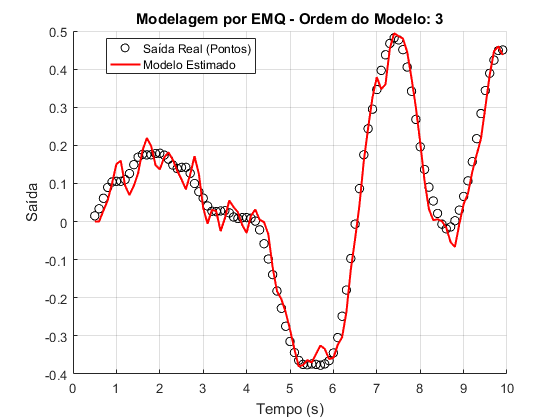
\includegraphics[height=5.4cm]{imgs/emq2-3.png} \quad
	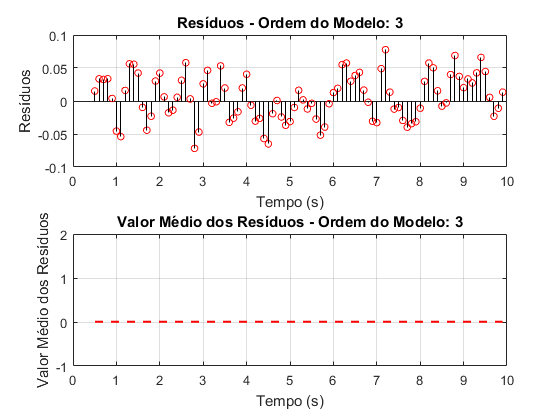
\includegraphics[height=5.4cm]{imgs/residuo2-3.png}
\caption{Resultados para $G_2(z)$ de ordem $3$} \label{fig13}
\end{center}
\end{figure}
\newpage
\noindent \textbf{Modelo de Ordem 4:}
\begin{equation*}
   y(k) = -0.98 \cdot u(k-1) + 4.21 \cdot u(k-2) - 7.37 \cdot u(k-3) + 5.10 \cdot u(k-4)\tag{4.4.2.4}
\end{equation*}
Os resíduos parecem continuar variando, mas podem estar começando a se aproximar de uma distribuição mais uniforme.

\begin{figure}[h!]
\begin{center}
	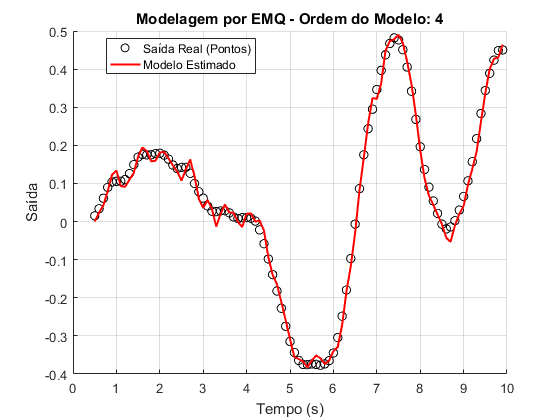
\includegraphics[height=5.4cm]{imgs/emq2-4.png} \quad
	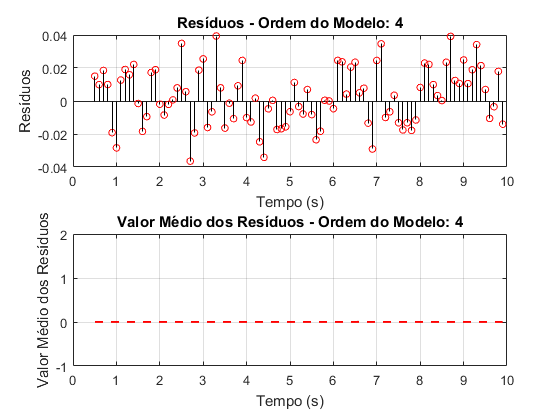
\includegraphics[height=5.4cm]{imgs/residuo2-4.png}
\caption{Resultados para $G_2(z)$ de ordem $4$} \label{fig14}
\end{center}
\end{figure}

\newpage
\noindent \textbf{Modelo de Ordem 5:}
\begin{equation*}
   y(k) = 0.45 \cdot u(k-1) - 1.76 \cdot u(k-2) + 3.37 \cdot u(k-3) - 4.21 \cdot u(k-4) + 3.15 \cdot u(k-5)\tag{4.4.2.5}
\end{equation*}
Os resíduos parecem ser os mais próximos de uma distribuição simétrica em torno de zero em comparação com os modelos anteriores.

\begin{figure}[h!]
\begin{center}
	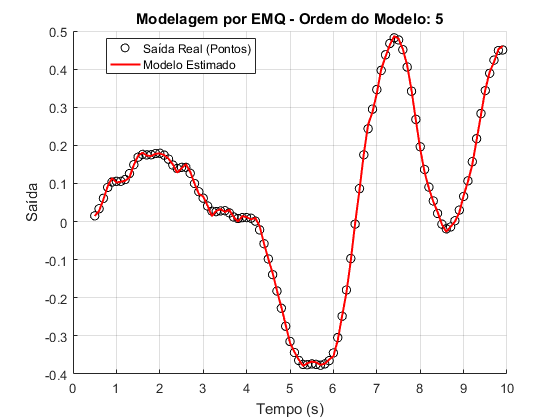
\includegraphics[height=5.4cm]{imgs/emq2-5.png} \quad
	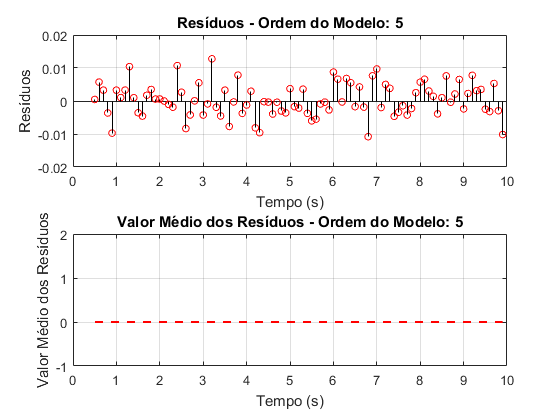
\includegraphics[height=5.4cm]{imgs/residuo2-5.png}
\caption{Resultados para $G_2(z)$ de ordem $5$} \label{fig15}
\end{center}
\end{figure}

Em geral, quanto maior a ordem do modelo, mais flexível ele é para se ajustar aos dados, mas também há um risco maior de sobreajuste (\textit{overfitting}). Portanto, a escolha da ordem do modelo deve ser cuidadosamente considerada com base na compreensão do domínio dos dados e na avaliação da qualidade do ajuste e dos resíduos.

\subsection{Parâmetros calculados com adição de ruído}

Os resultados para o procedimento apresentado em (\ref{3.5}) podem ser visualizados abaixo. Como descrito anteriormente, para cada iteração um valor diferente para o ruído foi calculado e o número total de iterações é $100$.

\subsubsection{Resultados para adição de ruído dinâmico}

Os valores calculados representam as estatísticas das médias e desvios padrão dos coeficientes estimados ($\theta$) ao longo das repetições usando o ruído dinâmico em cada iteração do \texttt{loop}. Os valores de média dos coeficientes tendem, neste caso, a convergir para $0.32$. 

Já para o desvio padrão, temos que os valores tendem a convergir para  $0.25$. Um desvio padrão menor indica que as médias dos coeficientes estão relativamente próximas da média geral ($0.32$), o que sugere que os coeficientes tendem a variar menos em relação à média geral.
\begin{figure}[h!]\label{fig16}
  \centering
  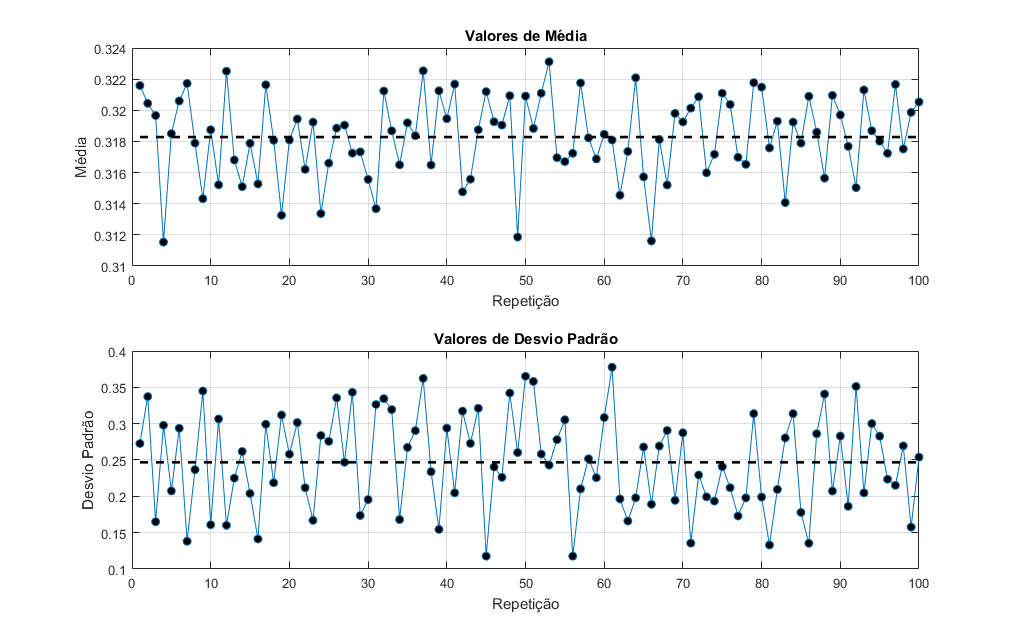
\includegraphics[width=\textwidth]{imgs/dinamico.png}
  \caption{Resultado para a adição do ruído dinâmico.}
\end{figure}

Isso significa que, mesmo com o ruído dinâmico variando em cada iteração, os coeficientes estimados estão se estabilizando em torno de um valor médio, e essa estabilidade é indicada pelo desvio padrão. Isso também sugere que o processo de estimação está sendo consistente e que os coeficientes não estão variando drasticamente em diferentes repetições.

\subsubsection{Resultados para adição de ruído estático}

Os valores calculados agora representam as estatísticas das médias e desvios padrão dos coeficientes estimados ($\theta$) ao longo das repetições usando o ruído estático em cada iteração do \texttt{loop}. Os coeficientes estimados tendem a convergir para um valor próximo de $0.33$.

Já para o desvio padrão, temos um valor maior ($1.26$), isso indica que as médias dos coeficientes têm uma variação mais significativa em relação à média geral ($0.33$) quando comparado ao caso do ruído dinâmico.
\begin{figure}[h!]\label{fig17}
  \centering
  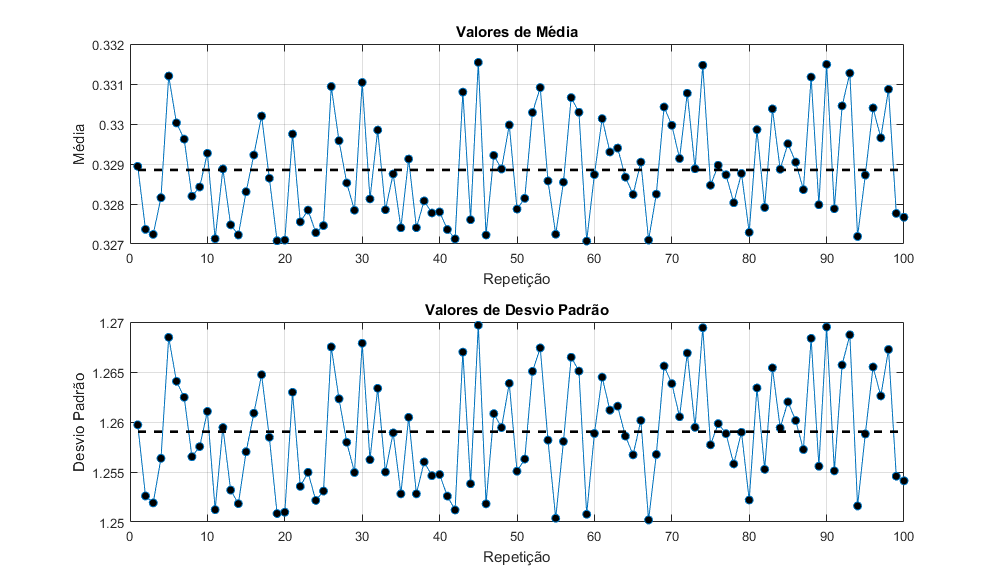
\includegraphics[width=\textwidth]{imgs/estatico.png}
  \caption{Resultado para a adição do ruído estático.}
\end{figure}
\newpage
Esses resultados sugerem que, ao usar ruído estático, os coeficientes estimados estão apresentando uma variação mais significativa em relação à média. Isso pode indicar que o processo de estimação está sendo influenciado pelo mesmo, resultando em coeficientes estimados mais dispersos. 
% O desvio padrão maior também indica que os coeficientes estão se afastando mais da média geral em comparação ao caso com ruído dinâmico, onde o desvio padrão era menor.

\subsection{Validação dos coeficientes encontrados}\label{4.6}

\subsubsection{Validação do sistema \ref{3.2.1} com a adição de ruído}

\begin{figure}[h!]
\centering

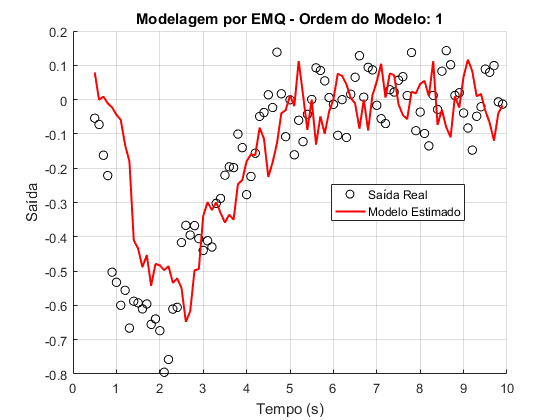
\includegraphics[height=3.4cm]{imgs/val-ordem1.png} \quad
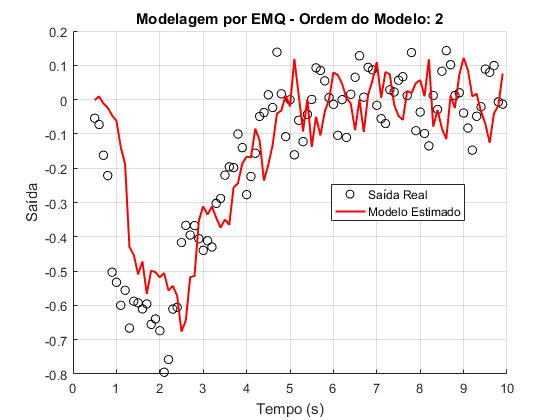
\includegraphics[height=3.4cm]{imgs/val-ordem2.png} \quad
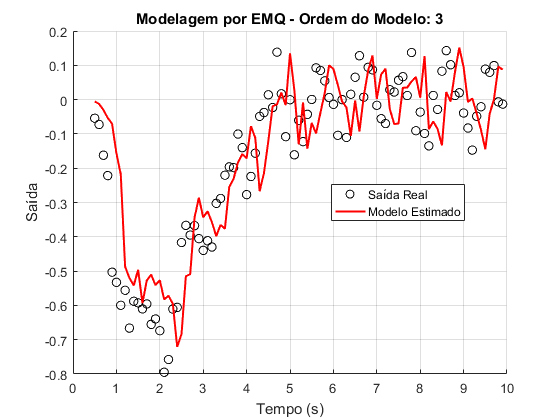
\includegraphics[height=3.4cm]{imgs/val-ordem3.png} \\

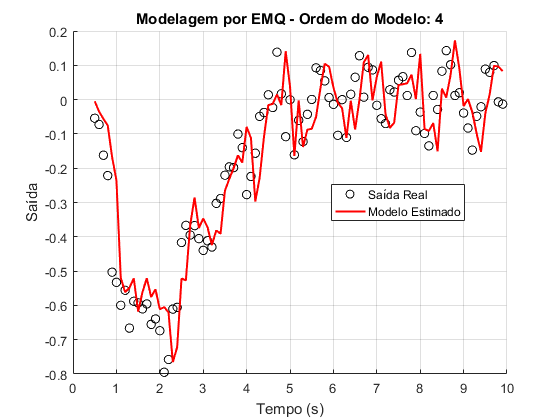
\includegraphics[height=3.4cm]{imgs/val-ordem4.png} \quad
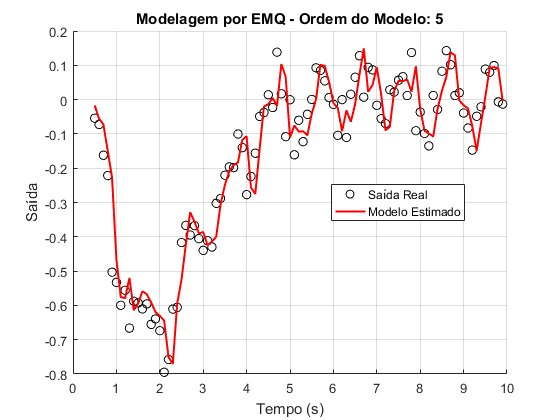
\includegraphics[height=3.4cm]{imgs/val-ordem5.png}

\caption{Saída dos Parâmetros estimados para a entrada senoidal.} \label{fig6}
\end{figure}

\begin{table}[h!]
    \centering
    \begin{tabular}{|c|c|c|c|}
        \hline
        \textbf{Ordem} & \textbf{SEQ} & \textbf{CCM} & \textbf{SNR} \\
        \hline
        1 & 2.87 & 0.51 & 14.01 \\ 
        2 & 2.38 & 0.60 & 14.37 \\ 
        3 & 1.74 & 0.70 & 14.80 \\ 
        4 & 1.03 & 0.83 & 15.23 \\ 
        5 & 0.60 & 0.90 & 15.48 \\ 
        \hline
    \end{tabular}
    \caption{Valores obtidos para os diferentes métodos utilizados.}
\end{table}

Para o modelo de \textbf{ordem 1}, observamos um valor relativamente alto de \textbf{SEQ}, indicando que o ajuste do modelo aos dados não é muito preciso. O \textbf{CCM} é em torno de 0.51, o que sugere uma correlação moderada entre as previsões do modelo e os dados reais. A \textbf{SNR} de 14.01 indica uma boa relação entre o sinal e o ruído, o que significa que o sinal de interesse é mais forte em comparação com o ruído.

O modelo de \textbf{ordem 2} apresenta uma melhoria no \textbf{SEQ} em comparação com o modelo de ordem 1, indicando um ajuste mais preciso aos dados. O \textbf{CCM} aumentou para 0.60, o que sugere uma correlação mais forte entre as previsões do modelo e os dados reais. A \textbf{SNR} também aumentou ligeiramente para 14.37, indicando uma relação sinal-ruído mais favorável.

O modelo de \textbf{ordem 3} apresenta uma queda significativa no \textbf{SEQ}, indicando um ajuste ainda melhor aos dados. O \textbf{CCM} aumentou para 0.70, o que sugere uma correlação mais forte entre as previsões do modelo e os dados reais. A \textbf{SNR} também aumentou ligeiramente para 14.80, indicando uma melhoria adicional na relação sinal-ruído.

O modelo de \textbf{ordem 4} apresenta um \textbf{SEQ} ainda menor, indicando um ajuste mais preciso aos dados. O \textbf{CCM} aumentou significativamente para 0.83, sugerindo uma correlação substancial entre as previsões do modelo e os dados reais. A \textbf{SNR} também aumentou para 15.23, indicando uma relação sinal-ruído muito favorável.

O modelo de \textbf{ordem 4} apresenta um \textbf{SEQ} ainda menor, indicando um ajuste mais preciso aos dados. O \textbf{CCM} aumentou significativamente para 0.83, sugerindo uma correlação substancial entre as previsões do modelo e os dados reais. A \textbf{SNR} também aumentou para 15.48, indicando uma relação sinal-ruído muito favorável.

Em resumo, os valores das métricas melhoraram à medida que a ordem do modelo aumentou. Isso sugere que modelos de ordem mais alta são mais capazes de capturar a relação entre o sinal de entrada e a saída do sistema, resultando em um ajuste mais preciso, maior correlação e melhor relação sinal-ruído. No entanto, a escolha da ordem do modelo deve ser feita com base em uma análise mais aprofundada para evitar o superajuste (\textit{overfitting}) aos dados de treinamento. 
\newpage
\subsubsection{Validação do sistema \ref{3.2.2} com a adição de ruído}

\begin{figure}[h!]
\centering

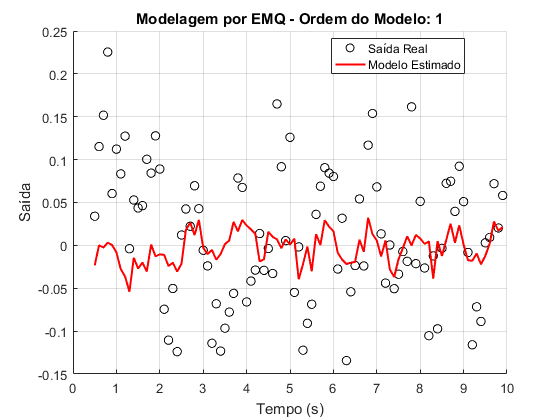
\includegraphics[height=3.4cm]{imgs/val-ordem11.png} \quad
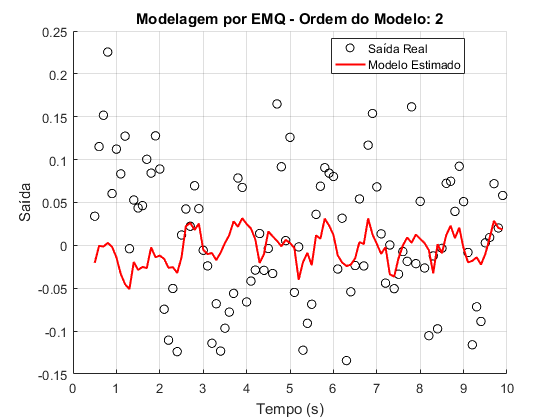
\includegraphics[height=3.4cm]{imgs/val-ordem22.png} \quad
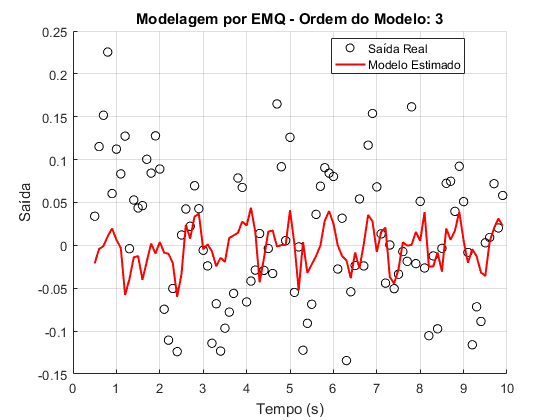
\includegraphics[height=3.4cm]{imgs/val-ordem33.png} \\

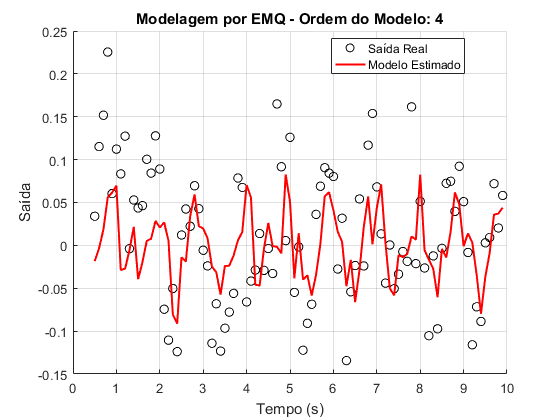
\includegraphics[height=3.4cm]{imgs/val-ordem44.png} \quad
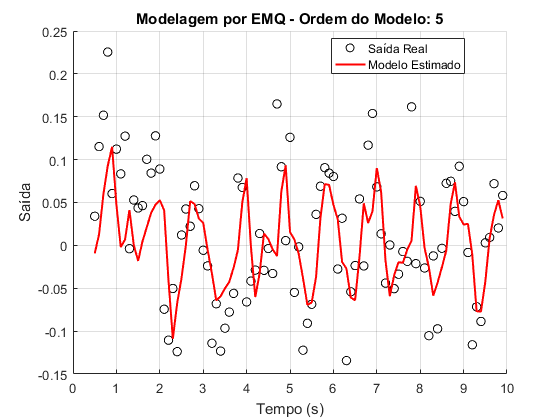
\includegraphics[height=3.4cm]{imgs/val-ordem55.png}

\caption{Saída dos Parâmetros estimados para a entrada senoidal.} \label{fig6}
\end{figure}

\begin{table}[h!]
    \centering
    \begin{tabular}{|c|c|c|c|}
        \hline
        \textbf{Ordem} & \textbf{SEQ} & \textbf{CCM} & \textbf{SNR} \\
        \hline
        1 & 0.55 & 0.03 & -8.22 \\
        2 & 0.55 & 0.03 & -8.02 \\ 
        3 & 0.53 & 0.07 & -6.15 \\ 
        4 & 0.44 & 0.22 & -1.95 \\
        5 & 0.38 & 0.33 & -0.38 \\
        \hline
    \end{tabular}
    \caption{Valores obtidos para os diferentes métodos utilizados.}
\end{table}

Para o modelo de \textbf{ordem 1}, observamos um valor moderado de \textbf{SEQ}, o que indica um ajuste razoável aos dados. No entanto, o baixo valor de \textbf{CCM} sugere uma correlação muito fraca entre as previsões do modelo e os dados reais. Além disso, a \textbf{SNR} negativa indica que o ruído é significativamente mais forte do que o sinal de interesse, o que pode prejudicar a confiabilidade das previsões do modelo.

O modelo de \textbf{ordem 2} apresenta resultados semelhantes ao modelo de ordem 1. O \textbf{SEQ} e o \textbf{CCM} são praticamente iguais. A \textbf{SNR} também permanece negativa, indicando que o ruído ainda é dominante em relação ao sinal de interesse.

No modelo de \textbf{ordem 3}, há uma melhoria significativa no \textbf{SEQ}, indicando um ajuste mais preciso aos dados em comparação com os modelos anteriores. O \textbf{CCM} também aumentou, sugerindo uma correlação um pouco mais forte. No entanto, a \textbf{SNR} ainda que menor, permanece é negativa, o que indica que o ruído ainda é um fator importante.

O modelo de \textbf{ordem 4} apresenta uma redução significativa no \textbf{SEQ}, indicando um ajuste mais preciso aos dados em comparação com os modelos anteriores. Além disso, o \textbf{CCM} aumentou substancialmente, sugerindo uma correlação mais forte entre as previsões do modelo e os dados reais. A \textbf{SNR}, embora ainda negativa, está mais próxima de zero, indicando que o sinal de interesse está começando a se destacar em relação ao ruído.

No modelo de \textbf{ordem 5}, o \textbf{SEQ} continua a diminuir, indicando um ajuste ainda mais preciso aos dados. O \textbf{CCM} também continua a aumentar, sugerindo uma correlação ainda mais forte. Além disso, a \textbf{SNR} está muito próxima de zero, o que significa que o sinal de interesse e o ruído estão em um equilíbrio próximo.

Em resumo, à medida que a ordem do modelo aumenta, observamos uma melhoria geral nas métricas de ajuste, correlação e relação sinal-ruído. No entanto, mesmo nos modelos de ordem mais alta, a SNR permanece negativa ou próxima de zero, indicando que o ruído ainda é uma consideração importante na modelagem e previsão do sistema.

\subsection{Resultados para os conjuntos 1 e 2}

\subsubsection{Modelos matemáticos ARX e simulação(conjunto 1)}

Os resultados gráficos dos modelos ARX encontrados para o \textbf{conjunto de dados 1} são apresentados abaixo.

\begin{figure}[h!]
\centering

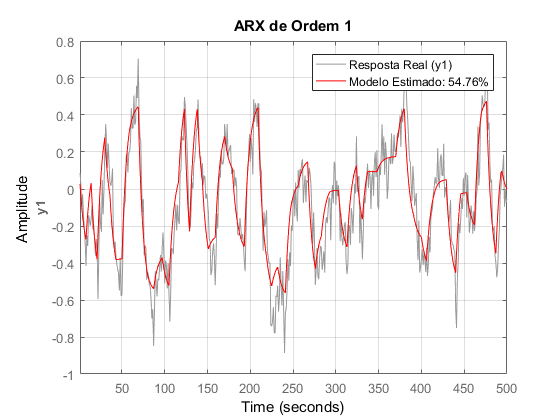
\includegraphics[height=3.4cm]{imgs/arx-1-1.png} \quad
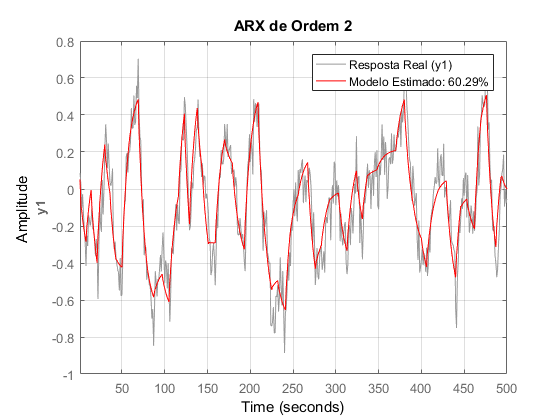
\includegraphics[height=3.4cm]{imgs/arx-1-2.png} \quad
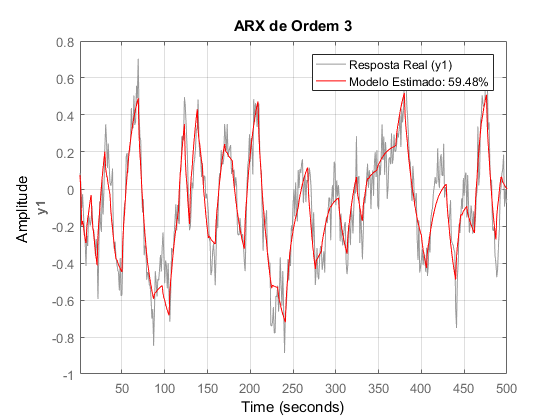
\includegraphics[height=3.4cm]{imgs/arx-1-3.png} \\

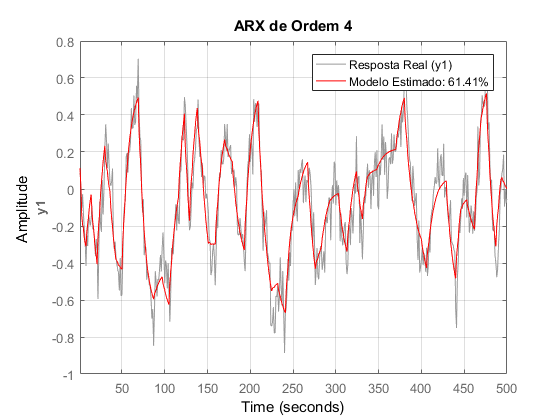
\includegraphics[height=3.4cm]{imgs/arx-1-4.png} \quad
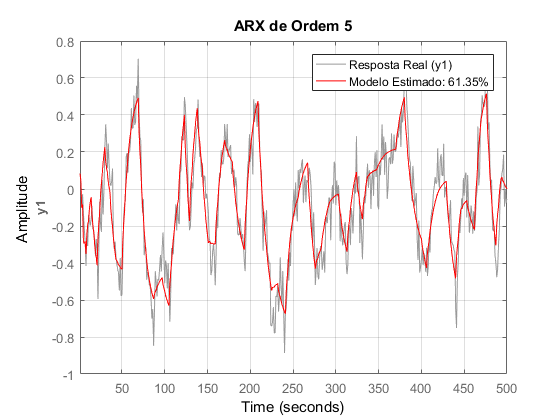
\includegraphics[height=3.4cm]{imgs/arx-1-5.png}

\caption{Resultados gráficos do modelo ARX para o conjunto 1.}
\end{figure}

Os modelos matemáticos estimados, com os coeficiente \mathcal{A} e \mathcal{B}, que geram as saídas presentes na Figura 21 são apresentados abaixo. Os modelos seguem a representação descrita na equação (\ref{3.7.1}).
\begin{itemize}
    \item Modelo de Ordem 1:
    \begin{equation*}
    y(t) = 0.84y(t-1) + 0.10u(t) + e(t)
    \end{equation*}
    
    \item Modelo de Ordem 2:
    \begin{equation*}
    y(t) = 0.61y(t-1) + 0.25y(t-2) + 0.11u(t) + e(t)
    \end{equation*}
    
    \item Modelo de Ordem 3:
    \begin{equation*}
    y(t) = 0.56y(t-1) + 0.09y(t-2) + 0.22y(t-3) + 0.13u(t) + e(t)
    \end{equation*}
    
    \item Modelo de Ordem 4:
    \begin{equation*}
    y(t) = 0.59y(t-1) + 0.10y(t-2) + 0.34y(t-3) - 0.17y(t-4) + 0.12u(t) + e(t)
    \end{equation*}
    
    \item Modelo de Ordem 5:
    \begin{align}
    y(t) = &0.60y(t-1) + 0.10y(t-2) + 0.33y(t-3) - 0.19y(t-4) + \nonumber \\
    & + 0.02y(t-5) + 0.12u(t) + e(t) \nonumber
    \end{align}
\end{itemize}

\subsubsection{Modelos matemáticos ARX e simulação(conjunto 2)}

Os resultados gráficos dos modelos ARX encontrados para o \textbf{conjunto de dados 2} são apresentados abaixo.

\begin{figure}[h!]
\centering

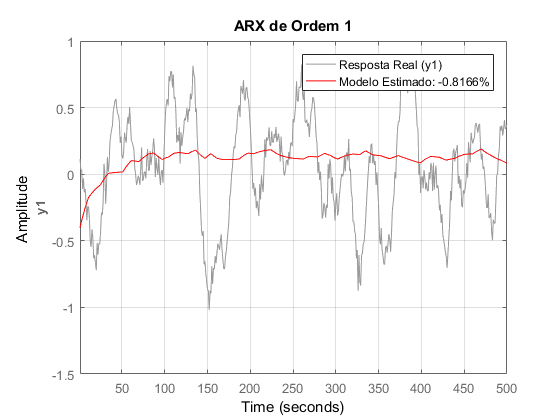
\includegraphics[height=3.4cm]{imgs/arx-2-1.png} \quad
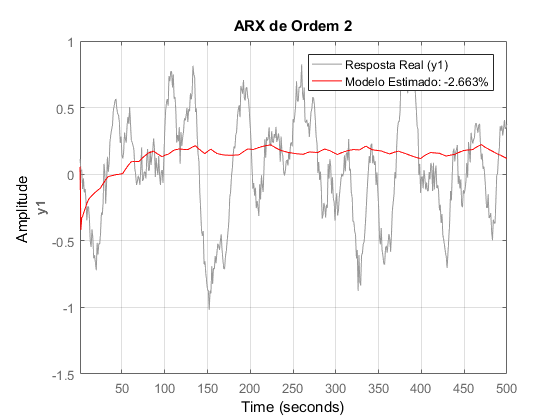
\includegraphics[height=3.4cm]{imgs/arx-2-2.png} \quad
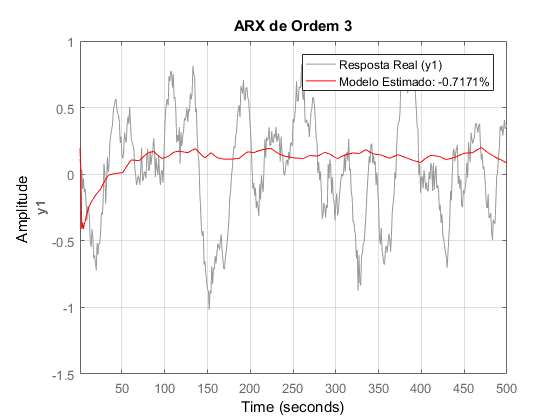
\includegraphics[height=3.4cm]{imgs/arx-2-3.png} \\

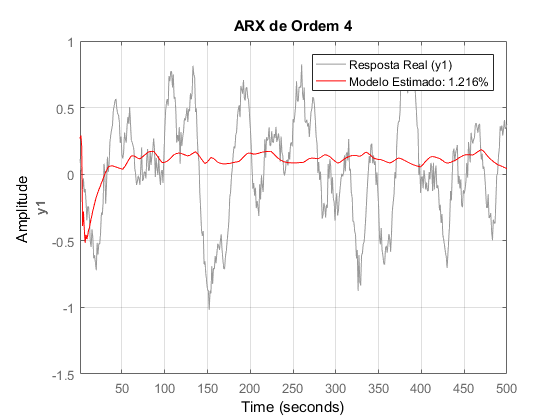
\includegraphics[height=3.4cm]{imgs/arx-2-4.png} \quad
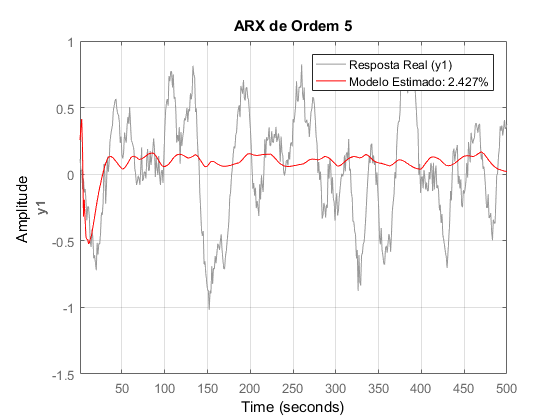
\includegraphics[height=3.4cm]{imgs/arx-2-5.png}

\caption{Resultados gráficos do modelo ARX para o conjunto 2.}
\end{figure}

Os modelos matemáticos estimados, com os coeficiente \mathcal{A} e \mathcal{B}, que geram as saídas presentes na Figura 22 são apresentados abaixo. Os modelos seguem a representação descrita na equação (\ref{3.7.1}).
\begin{itemize}
    \item Modelo de Ordem 1:
    \begin{equation*}
    y(t) = 0.96y(t-1) + 0.01u(t) + e(t)
    \end{equation*}
    
    \item Modelo de Ordem 2:
    \begin{equation*}
    y(t) = 0.83y(t-1) + 0.14y(t-2) + 0.01u(t) + e(t)
    \end{equation*}
    
    \item Modelo de Ordem 3:
    \begin{equation*}
    y(t) = 0.85y(t-1) + 0.27y(t-2) - 0.16y(t-3) + 0.01u(t) + e(t)
    \end{equation*}
    
    \item Modelo de Ordem 4:
    \begin{equation*}
    y(t) = 0.85y(t-1) + 0.27y(t-2) - 0.16y(t-3) + 0.01u(t) + e(t)
    \end{equation*}
    
    \item Modelo de Ordem 5:
    \begin{align}
    y(t) = &0.74y(t-1) + 0.36y(t-2) + 0.17y(t-3) - 0.13y(t-4) - \nonumber \\
    & - 0.21y(t-5) + 0.01u(t) + e(t) \nonumber
    \end{align}
\end{itemize}

\subsubsection{Resultante EMQ para os modelos ARX}

A Tabela abaixo apresenta os valores de EMQ para os 10 modelos testados durante as fases de estimação e validação.

\begin{table}[h!]
    \centering
    \label{tab:emq_results_arx}
    \begin{tabular}{|c|c|c|}
        \hline
        Ordem & Conjunto de Dados 1 & Conjunto de Dados 2 \\
        \hline
        1 & 0.23846 & 0.80968 \\
        2 & 0.28225 & 1.1486 \\
        3 & 0.31012 & 0.76965 \\
        4 & 0.29363 & 0.33846 \\
        5 & 0.29493 & 0.20308 \\
        \hline
    \end{tabular}
    \caption{Valores do EMQ para Modelos ARX nos Conjuntos de Dados 1 e 2}
\end{table}

\subsubsection{Justificativa da escolha do modelo ARX}

Com base nos valores da tabela, podemos justificar a escolha dos modelos ARX da seguinte forma: Para o \textbf{Conjunto 1}, observamos que o modelo ARX de ordem 1 apresenta o menor Erro Quadrático Médio (EMQ) em comparação com os outros modelos testados. Isso sugere que o modelo ARX de ordem 1 se ajusta melhor aos dados do Conjunto 1 e é a escolha preferida.
No caso do \textbf{Conjunto 2}, notamos que o modelo ARX de ordem 5 exibe o menor EMQ entre todas as ordens testadas. Isso indica que o modelo ARX de ordem 5 é o mais adequado para representar os dados do Conjunto 2 com maior precisão.

Portanto, a escolha dos modelos ARX é guiada pelos valores de EMQ em cada conjunto de dados. O modelo ARX de ordem 1 é selecionado para o Conjunto 1, enquanto o modelo ARX de ordem 5 é preferido para o Conjunto 2.

\subsubsection{Modelos matemáticos ARMAX e simulação(conjunto 1)}

Os resultados gráficos dos modelos ARMAX encontrados para o \textbf{conjunto de dados 1} são apresentados abaixo.

\begin{figure}[h!]
\centering

\includegraphics[height=3.4cm]{imgs/arm-1-1.png} \quad
\includegraphics[height=3.4cm]{imgs/arm-1-2.png} \quad
\includegraphics[height=3.4cm]{imgs/arm-1-3.png} \\

\includegraphics[height=3.4cm]{imgs/arm-1-4.png} \quad
\includegraphics[height=3.4cm]{imgs/arm-1-5.png}

\caption{Resultados gráficos do modelo ARMAX para o conjunto 1.}
\end{figure}

Os modelos matemáticos estimados, com os coeficiente \mathcal{A}, \mathcal{B} e \mathcal{C}, que geram as saídas presentes na Figura 23 são apresentados abaixo. Os modelos seguem a representação descrita na equação (\ref{3.7.2}).
\begin{itemize}
    \item Modelo de Ordem 1:
    \begin{equation*}
    y(t) = 0.90y(t-1) + 0.09u(t) - 0.58e(t)
    \end{equation*}
    
    \item Modelo de Ordem 2:
    \begin{equation*}
    y(t) = 1.29y(t-1) - 0.36y(t-2) + 0.06u(t) - 0.90e(t)
    \end{equation*}
    
    \item Modelo de Ordem 3:
    \begin{equation*}
    y(t) = 1.23y(t-1) - 0.21y(t-2) - 0.09y(t-3) + 0.06u(t) - 0.91e(t)
    \end{equation*}
    
    \item Modelo de Ordem 4:
    \begin{align}
    y(t) = &1.19y(t-1) - 0.29y(t-2) + 0.21y(t-3) - 0.18y(t-4) + \nonumber\\
    & + 0.06u(t) - 0.89e(t) \nonumber
    \end{align}
    
    \item Modelo de Ordem 5:
    \begin{align}
    y(t) = &1.23y(t-1) - 0.32y(t-2) + 0.27y(t-3) - 0.39y(t-4) +\nonumber \\
    & + 0.13y(t-5) + 0.05u(t) - 0.91e(t) \nonumber
    \end{align}
\end{itemize}

\subsubsection{Modelos matemáticos ARMAX e simulação(conjunto 2)}

Os resultados gráficos dos modelos ARMAX encontrados para o \textbf{conjunto de dados 2} são apresentados abaixo.

\begin{figure}[h!]
\centering

\includegraphics[height=3.4cm]{imgs/arm-2-1.png} \quad
\includegraphics[height=3.4cm]{imgs/arm-2-2.png} \quad
\includegraphics[height=3.4cm]{imgs/arm-2-3.png} \\

\includegraphics[height=3.4cm]{imgs/arm-2-4.png} \quad
\includegraphics[height=3.4cm]{imgs/arm-2-5.png}

\caption{Resultados gráficos do modelo ARMAX para o conjunto 2.}
\end{figure}

Os modelos matemáticos estimados, com os coeficiente \mathcal{A}, \mathcal{B} e \mathcal{C}, que geram as saídas presentes na Figura 24 são apresentados abaixo. Os modelos seguem a representação descrita na equação (\ref{3.7.2}).
\begin{itemize}
    \item Modelo de Ordem 1:
    \begin{equation*}
    y(t) = 0.97y(t-1) + 0.01u(t) - 0.10e(t)
    \end{equation*}
    
    \item Modelo de Ordem 2:
    \begin{equation*}
    y(t) = 1.91y(t-1) - 0.92y(t-2) + 0.00u(t) - 0.90e(t)
    \end{equation*}
    
    \item Modelo de Ordem 3:
    \begin{equation*}
    y(t) = 1.50y(t-1) - 0.18y(t-2) - 0.34y(t-3) + 0.00u(t) - 0.72e(t)
    \end{equation*}
    
    \item Modelo de Ordem 4:
    \begin{align}
    y(t) = &1.25y(t-1) - 0.03y(t-2) - 0.00y(t-3) - 0.25y(t-4) + \nonumber\\
    & + 0.01u(t) - 0.52e(t) \nonumber
    \end{align}
    
    \item Modelo de Ordem 5:
    \begin{align}
    y(t) = &1.09y(t-1) + 0.08y(t-2) + 0.05y(t-3) - 0.15y(t-4) -\nonumber \\
    & - 0.12y(t-5) + 0.01u(t) - 0.38e(t) \nonumber
    \end{align}
\end{itemize}

\subsubsection{Resultante EMQ para os modelos ARMAX}

A Tabela abaixo apresenta os valores de EMQ para os 10 modelos testados durante as fases de estimação e validação.

\begin{table}[h!]
    \centering
    \label{tab:emq_results_armax}
    \begin{tabular}{|c|c|c|}
        \hline
        Ordem & Conjunto de Dados 1 & Conjunto de Dados 2 \\
        \hline
        1 & 0.29681 & 1.0563 \\
        2 & 0.27854 & 0.11792 \\
        3 & 0.27803 & 0.13838 \\
        4 & 0.28246 & 0.14864 \\
        5 & 0.27981 & 0.15112 \\
        \hline
    \end{tabular}
    \caption{Valores do EMQ para Modelos ARMAX nos Conjuntos de Dados 1 e 2}
\end{table}
\subsubsection{Justificativa da escolha do modelo ARMAX}

Com base nos valores da tabela, podemos justificar a escolha dos modelos ARMAX da seguinte forma: No \textbf{Conjunto de Dados 1}, observamos que os valores de EMQ variam ligeiramente entre as diferentes ordens dos modelos testados. O valor mínimo de é obtido para a \textbf{ordem 3}. A medida que a ordem aumenta, o EMQ tende a aumentar ligeiramente. Isso sugere que a ordem 3 pode ser a escolha preferida para o Conjunto de Dados 1. No \textbf{Conjunto de Dados 2}, há uma variação mais significativa nos valores de EMQ em relação à ordem dos modelos ARMAX. O valor mínimo de EMQ é obtido para a \textbf{ordem 2}, seguido pela ordem 3. As demais ordens têm valores de EMQ mais elevados. Isso sugere que o modelo ARMAX de ordem 2 é a escolha mais adequada para o Conjunto de Dados 2, uma vez que ele apresenta o menor erro médio quadrático em comparação com as outras ordens.

\subsection{Resultados para os conjuntos 3 e 4}

\subsubsection{Modelos matemáticos ARX e simulação(conjunto 3)}

Os resultados gráficos dos modelos ARX encontrados para o \textbf{conjunto de dados 3} são apresentados abaixo.

\begin{figure}[h!]
\centering

\includegraphics[height=3.4cm]{imgs/arx-3-1.png} \quad
\includegraphics[height=3.4cm]{imgs/arx-3-2.png} \quad
\includegraphics[height=3.4cm]{imgs/arx-3-3.png} \\

\includegraphics[height=3.4cm]{imgs/arx-3-4.png} \quad
\includegraphics[height=3.4cm]{imgs/arx-3-5.png}

\caption{Resultados gráficos do modelo ARX para o conjunto 3.}
\end{figure}

Os modelos matemáticos estimados, com os coeficiente \mathcal{A} e \mathcal{B}, que geram as saídas presentes na Figura 25 são apresentados abaixo. Os modelos seguem a representação descrita na equação (\ref{3.7.1}).
\begin{itemize}
    \item Modelo de Ordem 1:
    \begin{equation*}
    y(t) = 0.34y(t-1) + 1.30u(t) + e(t)
    \end{equation*}
    
    \item Modelo de Ordem 2:
    \begin{equation*}
    y(t) = 0.20y(t-1) + 0.18y(t-2) + 1.24u(t) + e(t)
    \end{equation*}
    
    \item Modelo de Ordem 3:
    \begin{equation*}
    y(t) = 0.20y(t-1) + 0.14y(t-2) + 0.07y(t-3) + 1.16u(t) + e(t)
    \end{equation*}
    
    \item Modelo de Ordem 4:
    \begin{equation*}
    y(t) = 0.17y(t-1) + 0.16y(t-2) + 0.08y(t-3) + 0.00y(t-4) + 1.16u(t) + e(t)
    \end{equation*}
    
    \item Modelo de Ordem 5:
    \begin{align*}
    y(t) &= 0.17y(t-1) + 0.16y(t-2) + 0.06y(t-3) - 0.03y(t-4) +\\
    &+ 0.06y(t-5) + 1.16u(t) + e(t)
    \end{align*}
\end{itemize}

\subsubsection{Modelos matemáticos ARX e simulação(conjunto 4)}

Os resultados gráficos dos modelos ARX encontrados para o \textbf{conjunto de dados 4} são apresentados abaixo.
\begin{figure}[h!]
\centering

\includegraphics[height=3.4cm]{imgs/arx-4-1.png} \quad
\includegraphics[height=3.4cm]{imgs/arx-4-2.png} \quad
\includegraphics[height=3.4cm]{imgs/arx-4-3.png} \\

\includegraphics[height=3.4cm]{imgs/arx-4-4.png} \quad
\includegraphics[height=3.4cm]{imgs/arx-4-5.png}

\caption{Resultados gráficos do modelo ARX para o conjunto 4.}
\end{figure}

Os modelos matemáticos estimados, com os coeficiente \mathcal{A} e \mathcal{B}, que geram as saídas presentes na Figura 26 são apresentados abaixo. Os modelos seguem a representação descrita na equação (\ref{3.7.1}).

\begin{itemize}
    \item Modelo de Ordem 1:
    \begin{equation*}
    y(t) = 0.36y(t-1) + 0.37u(t) + e(t)
    \end{equation*}
    
    \item Modelo de Ordem 2:
    \begin{equation*}
    y(t) = 0.16y(t-1) + 0.33y(t-2) + 0.34u(t) + e(t)
    \end{equation*}
    
    \item Modelo de Ordem 3:
    \begin{equation*}
    y(t) = 0.16y(t-1) + 0.33y(t-2) + 0.01y(t-3) + 0.34u(t) + e(t)
    \end{equation*}
    
    \item Modelo de Ordem 4:
    \begin{equation*}
    y(t) = 0.16y(t-1) + 0.33y(t-2) + 0.01y(t-3) + 0.00y(t-4) + 0.34u(t) + e(t)
    \end{equation*}
    
    \item Modelo de Ordem 5:
    \begin{align*}
    y(t) &= 0.16y(t-1) + 0.33y(t-2) - 0.00y(t-3) - 0.01y(t-4) - \\
    &- 0.01y(t-5) + 0.34u(t) + e(t)
    \end{align*}
\end{itemize}

\subsubsection{Resultante EMQ para os modelos ARX}

A Tabela abaixo apresenta os valores de EMQ para os 10 modelos testados durante as fases de estimação e validação.
\begin{table}[h!]
    \centering
    \label{tab:emq_results_armax}
    \begin{tabular}{|c|c|c|}
        \hline
        Ordem & Conjunto de Dados 3 & Conjunto de Dados 4 \\
        \hline
        1 & 3.2763 & 0.22463 \\
        2 & 3.3623 & 0.47196 \\
        3 & 3.346 & 0.47603 \\
        4 & 3.3085 & 0.47733 \\
        5 & 3.3263 & 0.4808 \\
        \hline
    \end{tabular}
    \caption{Valores do EMQ para Modelos ARX nos Conjuntos de Dados 3 e 4}
\end{table}
\subsubsection{Resultante do comportamento dos Regressores ARX}

Os resultados gráficos do comportamento dos regressores para os 10 modelos testados durante as fases de estimação e validação são apresentados abaixo.
\begin{figure}[h!]
\centering

\includegraphics[height=3.4cm]{imgs/arx-11-r.png} \quad
\includegraphics[height=3.4cm]{imgs/arx-22-r.png} \quad
\includegraphics[height=3.4cm]{imgs/arx-33-r.png} \\

\includegraphics[height=3.4cm]{imgs/arx-44-r.png} \quad
\includegraphics[height=3.4cm]{imgs/arx-55-r.png}

\caption{Comportamento dos regressores do modelo ARX para o conjunto 3.}
\end{figure}

Podemos notar, através do gráfico de variância que os valores dos regressores apresentam um comportamento aceitável para atestar que os sistemas estimados para o \textbf{conjunto de dados 3} \textbf{não são variantes no tempo}, uma vez que os mesmos estão muito próximos do valor médio.

\begin{figure}[h!]
\centering

\includegraphics[height=3.4cm]{imgs/arx-5-r.png} \quad
\includegraphics[height=3.4cm]{imgs/arx-4-r.png} \quad
\includegraphics[height=3.4cm]{imgs/arx-3-r.png} \\

\includegraphics[height=3.4cm]{imgs/arx-2-r.png} \quad
\includegraphics[height=3.4cm]{imgs/arx-1-r.png}

\caption{Comportamento dos regressores do modelo ARX para o conjunto 4.}
\end{figure}

Podemos notar, através do gráfico de variância que os valores dos regressores apresentam um comportamento aceitável para atestar que os sistemas estimados para o \textbf{conjunto de dados 4} \textbf{não são variantes no tempo}, uma vez que os mesmos estão muito próximos do valor médio.

\subsubsection{Justificativa da escolha do modelo ARX}

Com base nos valores da tabela de Erro Quadrático Médio (EMQ), podemos justificar a escolha do melhor modelo da seguinte maneira: No \textbf{Conjunto de Dados 3}, observamos que os valores de EMQ aumentam gradualmente à medida que a ordem dos modelos ARX aumenta. O valor mínimo de EMQ é obtido para a \textbf{ordem 1}. À medida que a ordem aumenta, os valores de EMQ continuam aumentando, sugerindo que modelos mais complexos podem estar se ajustando demais aos dados de treinamento, resultando em piores desempenhos de predição em dados não vistos. Portanto, a escolha do melhor modelo para o Conjunto de Dados 3 seria o modelo ARX de ordem 1, devido ao menor valor de EMQ, indicando uma melhor capacidade de generalização.

No \textbf{Conjunto de Dados 4}, também observamos um aumento nos valores de EMQ à medida que a ordem dos modelos aumenta. O valor mínimo de EMQ é obtido novamente para a \textbf{ordem 1}. Assim como no Conjunto de Dados 3, as ordens mais altas têm valores de EMQ maiores. Isso reforça a ideia de que escolher um modelo mais simples, como o de ordem 1, pode ser mais vantajoso, uma vez que ele pode evitar o \textit{overfitting} e proporcionar uma melhor generalização para dados não vistos.

\subsubsection{Modelos matemáticos ARMAX e simulação(conjunto 3)}

Os resultados gráficos dos modelos ARMAX encontrados para o \textbf{conjunto de dados 3} são apresentados abaixo.

\begin{figure}[h!]
\centering

\includegraphics[height=3.4cm]{imgs/arm-3-1.png} \quad
\includegraphics[height=3.4cm]{imgs/arm-3-2.png} \quad
\includegraphics[height=3.4cm]{imgs/arm-3-3.png} \\

\includegraphics[height=3.4cm]{imgs/arm-3-4.png} \quad
\includegraphics[height=3.4cm]{imgs/arm-3-5.png}

\caption{Resultados gráficos do modelo ARMAX para o conjunto 3.}
\end{figure}

Os modelos matemáticos estimados, com os coeficiente \mathcal{A}, \mathcal{B} e \mathcal{C}, que geram as saídas presentes na Figura 29 são apresentados abaixo. Os modelos seguem a representação descrita na equação (\ref{3.7.2}).
\begin{itemize}
    \item Modelo de Ordem 1:
    \begin{equation*}
    y(t) = 0.54y(t-1) + 0.92u(t) - 0.52e(t)
    \end{equation*}
    
    \item Modelo de Ordem 2:
    \begin{equation*}
    y(t) = 0.53y(t-1) - 0.01y(t-2) + 0.96u(t) - 0.52e(t)
    \end{equation*}
    
    \item Modelo de Ordem 3:
    \begin{equation*}
    y(t) = 0.57y(t-1) + 0.01y(t-2) - 0.02y(t-3) + 0.89u(t) - 0.53e(t)
    \end{equation*}
    
    \item Modelo de Ordem 4:
    \begin{align}
    y(t) &= 0.55y(t-1) + 0.04y(t-2) + 0.00y(t-3) - 0.03y(t-4) \nonumber\\
    &+ 0.89u(t) - 0.52e(t) \nonumber
    \end{align}
    
    \item Modelo de Ordem 5:
    \begin{align}
    y(t) &= 0.55y(t-1) + 0.04y(t-2) + 0.00y(t-3) - 0.06y(t-4)\nonumber \\
    &+ 0.02y(t-5) + 0.89u(t) - 0.52e(t) \nonumber
    \end{align}
\end{itemize}


\subsubsection{Modelos matemáticos ARMAX e simulação(conjunto 4)}
Os resultados gráficos dos modelos ARMAX encontrados para o \textbf{conjunto de dados 3} são apresentados abaixo.

\begin{figure}[h!]
\centering

\includegraphics[height=3.4cm]{imgs/arm-4-1.png} \quad
\includegraphics[height=3.4cm]{imgs/arm-4-2.png} \quad
\includegraphics[height=3.4cm]{imgs/arm-4-3.png} \\

\includegraphics[height=3.4cm]{imgs/arm-4-4.png} \quad
\includegraphics[height=3.4cm]{imgs/arm-4-5.png}

\caption{Resultados gráficos do modelo ARMAX para o conjunto 4.}
\end{figure}

Os modelos matemáticos estimados, com os coeficiente \mathcal{A}, \mathcal{B} e \mathcal{C}, que geram as saídas presentes na Figura 30 são apresentados abaixo. Os modelos seguem a representação descrita na equação (\ref{3.7.2}).
\begin{itemize}
    \item Modelo de Ordem 1:
    \begin{equation*}
    y(t) = 0.54y(t-1) + 0.92u(t) - 0.52e(t)
    \end{equation*}
    
    \item Modelo de Ordem 2:
    \begin{equation*}
    y(t) = 0.53y(t-1) - 0.01y(t-2) + 0.96u(t) - 0.52e(t)
    \end{equation*}
    
    \item Modelo de Ordem 3:
    \begin{equation*}
    y(t) = 0.57y(t-1) + 0.01y(t-2) - 0.02y(t-3) + 0.89u(t) - 0.53e(t)
    \end{equation*}
    
    \item Modelo de Ordem 4:
    \begin{align}
    y(t) &= 0.55y(t-1) + 0.04y(t-2) + 0.00y(t-3) - 0.03y(t-4) \nonumber\\
    &+ 0.89u(t) - 0.52e(t) \nonumber
    \end{align}
    
    \item Modelo de Ordem 5:
    \begin{align}
    y(t) &= 0.55y(t-1) + 0.04y(t-2) + 0.00y(t-3) - 0.06y(t-4)\nonumber \\
    &+ 0.02y(t-5) + 0.89u(t) - 0.52e(t) \nonumber
    \end{align}
\end{itemize}

\subsubsection{Resultante EMQ para os modelos ARMAX}

A Tabela abaixo apresenta os valores de EMQ para os 10 modelos testados durante as fases de estimação e validação.

\begin{table}[h!]
    \centering
    \label{tab:emq_results_armax}
    \begin{tabular}{|c|c|c|}
        \hline
        Ordem & Conjunto de Dados 3 & Conjunto de Dados 4 \\
        \hline
        1 & 3.0398 & 0.44987 \\
        2 & 3.042 & 0.44118 \\
        3 & 3.0338 & 0.43517 \\
        4 & 3.0226 & 0.4354 \\
        5 & 3.0287 & 0.43491 \\
        \hline
    \end{tabular}
    \caption{Valores do EMQ para Modelos ARMAX nos Conjuntos de Dados 3 e 4}
\end{table}

\subsubsection{Resultante do comportamento dos Regressores ARMAX}

Os resultados gráficos do comportamento dos regressores para os 10 modelos testados durante as fases de estimação e validação são apresentados abaixo.
\begin{figure}[h!]
\centering

\includegraphics[height=3.4cm]{imgs/arm-11-r.png} \quad
\includegraphics[height=3.4cm]{imgs/arm-22-r.png} \quad
\includegraphics[height=3.4cm]{imgs/arm-33-r.png} \\

\includegraphics[height=3.4cm]{imgs/arm-44-r.png} \quad
\includegraphics[height=3.4cm]{imgs/arm-55-r.png}

\caption{Comportamento dos regressores do modelo ARX para o conjunto 3.}
\end{figure}

Podemos notar, através do gráfico de variância que os valores dos regressores, para os modelos de ordem 3, 4 e 5 apresentam um comportamento aceitável para atestar que o sistema estimado para o \textbf{conjunto de dados 3} \textbf{não é variante no tempo}, uma vez que os mesmo estão muito próximos do valor médio. Contudo, os valores para os modelos de ordem 1 e 2, apresentam uma maior instabilidade, desta forma, podemos atestar que os modelos em questão são variantes no tempo.

\begin{figure}[h!]
\centering

\includegraphics[height=3.4cm]{imgs/arm-1-r.png} \quad
\includegraphics[height=3.4cm]{imgs/amr-2-r.png} \quad
\includegraphics[height=3.4cm]{imgs/arm-3-r.png} \\

\includegraphics[height=3.4cm]{imgs/arm-4-r.png} \quad
\includegraphics[height=3.4cm]{imgs/arm-5-r.png}

\caption{Comportamento dos regressores do modelo ARX para o conjunto 4.}
\end{figure}

Podemos notar, através do gráfico de variância que os valores dos regressores apresentam um comportamento aceitável para atestar que os sistemas estimados para o \textbf{conjunto de dados 4} \textbf{não são variantes no tempo}, uma vez que os mesmos estão muito próximos do valor médio.

\subsubsection{Justificativa da escolha do modelo ARMAX}

Com base nos valores da tabela de Erro Quadrático Médio (EMQ) para os conjuntos de dados 3 e 4, podemos justificar a escolha do melhor modelo da seguinte forma: No \textbf{Conjunto de Dados 3}, observamos que os valores de EMQ apresentam pouca variação à medida que a ordem dos modelos ARMAX aumenta. Isso sugere que a complexidade do modelo não está impactando significativamente o desempenho de predição. Desta forma, usando como critério o a variação temporal, podemos atestar que o modelo de \textbf{ordem 3} se adéqua para estimar o sistema.

No \textbf{Conjunto de Dados 4}, também observamos uma variação relativamente pequena nos valores de EMQ à medida que a ordem aumenta. Isso indica que, sem informações adicionais, escolher o melhor modelo com base apenas nos valores de EMQ pode não ser conclusivo. Contudo, levando em conta a variação temporal dos modelos estimados, podemos adotar o modelo de \textbf{ordem 1} para para simular o sistema real.

%Conclusão
\newpage
\section{Conclusão}

%Bibliográfia
\newpage
\bibliographystyle{ieeetr}
\bibliography{bibliografia}
\nocite{*}

%Apêndice
\newpage
\begin{flushleft}
\Large
\textbf{Apêndices}
\end{flushleft}

\end{document}
